\documentclass[12pt,a4paper,]{report}
\usepackage{lmodern}
\usepackage{setspace}
\setstretch{1.5}
\usepackage{amssymb,amsmath}
\usepackage{ifxetex,ifluatex}
\usepackage{fixltx2e} % provides \textsubscript
\ifnum 0\ifxetex 1\fi\ifluatex 1\fi=0 % if pdftex
  \usepackage[T1]{fontenc}
  \usepackage[utf8]{inputenc}
\else % if luatex or xelatex
  \ifxetex
    \usepackage{mathspec}
  \else
    \usepackage{fontspec}
  \fi
  \defaultfontfeatures{Ligatures=TeX,Scale=MatchLowercase}
    \setmainfont[]{Calibri}
\fi
% use upquote if available, for straight quotes in verbatim environments
\IfFileExists{upquote.sty}{\usepackage{upquote}}{}
% use microtype if available
\IfFileExists{microtype.sty}{%
\usepackage{microtype}
\UseMicrotypeSet[protrusion]{basicmath} % disable protrusion for tt fonts
}{}
\usepackage[left=4cm,right=2.5cm,top=2.5cm,bottom=2.5cm]{geometry}
\usepackage{hyperref}
\hypersetup{unicode=true,
            pdfborder={0 0 0},
            breaklinks=true}
\urlstyle{same}  % don't use monospace font for urls
\usepackage{natbib}
\bibliographystyle{apalike}
\usepackage{longtable,booktabs}
\usepackage{graphicx,grffile}
\makeatletter
\def\maxwidth{\ifdim\Gin@nat@width>\linewidth\linewidth\else\Gin@nat@width\fi}
\def\maxheight{\ifdim\Gin@nat@height>\textheight\textheight\else\Gin@nat@height\fi}
\makeatother
% Scale images if necessary, so that they will not overflow the page
% margins by default, and it is still possible to overwrite the defaults
% using explicit options in \includegraphics[width, height, ...]{}
\setkeys{Gin}{width=\maxwidth,height=\maxheight,keepaspectratio}
\IfFileExists{parskip.sty}{%
\usepackage{parskip}
}{% else
\setlength{\parindent}{0pt}
\setlength{\parskip}{6pt plus 2pt minus 1pt}
}
\setlength{\emergencystretch}{3em}  % prevent overfull lines
\providecommand{\tightlist}{%
  \setlength{\itemsep}{0pt}\setlength{\parskip}{0pt}}
\setcounter{secnumdepth}{5}
% Redefines (sub)paragraphs to behave more like sections
\ifx\paragraph\undefined\else
\let\oldparagraph\paragraph
\renewcommand{\paragraph}[1]{\oldparagraph{#1}\mbox{}}
\fi
\ifx\subparagraph\undefined\else
\let\oldsubparagraph\subparagraph
\renewcommand{\subparagraph}[1]{\oldsubparagraph{#1}\mbox{}}
\fi

%%% Use protect on footnotes to avoid problems with footnotes in titles
\let\rmarkdownfootnote\footnote%
\def\footnote{\protect\rmarkdownfootnote}

%%% Change title format to be more compact
\usepackage{titling}

% Create subtitle command for use in maketitle
\newcommand{\subtitle}[1]{
  \posttitle{
    \begin{center}\large#1\end{center}
    }
}

\setlength{\droptitle}{-2em}
  \title{}
  \pretitle{\vspace{\droptitle}}
  \posttitle{}
  \author{}
  \preauthor{}\postauthor{}
  \date{}
  \predate{}\postdate{}

\usepackage{booktabs}

\usepackage[table]{xcolor}
\definecolor{lightgrey}{gray}{0.85}

\usepackage{pdfpages}

\usepackage{rotating}

\usepackage{multirow}

\usepackage{array}

\usepackage{setspace}
\onehalfspacing

\usepackage{gensymb}

\usepackage{chngcntr}

\usepackage{appendix}

\usepackage{fancyhdr}

\usepackage{caption}

\usepackage{float}

\pagenumbering{roman}

\usepackage{amsthm}
\newtheorem{theorem}{Theorem}[chapter]
\newtheorem{lemma}{Lemma}[chapter]
\theoremstyle{definition}
\newtheorem{definition}{Definition}[chapter]
\newtheorem{corollary}{Corollary}[chapter]
\newtheorem{proposition}{Proposition}[chapter]
\theoremstyle{definition}
\newtheorem{example}{Example}[chapter]
\theoremstyle{definition}
\newtheorem{exercise}{Exercise}[chapter]
\theoremstyle{remark}
\newtheorem*{remark}{Remark}
\newtheorem*{solution}{Solution}
\begin{document}

\thispagestyle{empty}
\begin{center}

\includegraphics{logos/tuoslogo_cmyk_hi.jpg}
\vspace{1.5cm}
 {\Huge\bfseries \\The impacts of tropical forest degradation and conversion on resilience to climate change\par}
 \vspace{1.5cm}
 {\Large By:\\ Rebecca Anne Senior\par}
 \vspace{1.5cm}
 {A thesis submitted in partial fulfilment of the requirements for the degree of\\ Doctor of Philosophy\par}
 \vspace{2cm}\bfseries
 The University of Sheffield\\
 Faculty of Science\\
 Department of Animal and Plant Sciences\par
 \vfill
 {\large {\normalfont Submission Date\par}}
\end{center}

\setlength{\abovedisplayskip}{-5pt}
\setlength{\abovedisplayshortskip}{-5pt}


\nocite{gonzalez_del_pliego_unpublished, 
gonzalez-di_pierro_effects2011,
  goode_unpublished,
  goode_seed2009,
  ibanez_sharp2013,
  lebrija-trejos_environmental2011,
  negrete-yankelevich_successional2007,
  santos_interaccion2011,
  santos_insect2012,
  sonnleitner_microclimatic2009,
  wood_no2008,
  yashiro_effects2008,
  adachi_differences2006,
  hardwick_aboveground2016,
  hardwick_relationship2015,
  klein_predatorprey2002,
  wangluk_role2013,
  werner_n2o2006,
  holl_factors1999,
  liu_exotic2002,
  king_ants1998,
  badejo_response2004,
  campos_response2006,
  badejo_seasonal1990,
  furukawa_effect2005}

{
\setcounter{tocdepth}{1}
\tableofcontents
}
\listoftables
\listoffigures
\chapter*{Abstract}\label{abstract}
\addcontentsline{toc}{chapter}{Abstract}

Stuff about tropical forests being important and blah blah blah.

\pagebreak

\chapter*{Acknowledgements}\label{acknowledgements}
\addcontentsline{toc}{chapter}{Acknowledgements}

Thanks everyone for being alright.

\pagebreak

\chapter*{Author's declaration}\label{authors-declaration}
\addcontentsline{toc}{chapter}{Author's declaration}

I did all this shit yo.

\pagebreak

\pagestyle{fancyplain} \fancyhf{}
\fancyhead[R]{\nouppercase\chaptername \space \thechapter}
\fancyfoot[R]{\thepage} \pagenumbering{arabic}

\chapter{General introduction}\label{general-introduction}

\begin{figure}[!htb]
\centering
\includegraphics[width=15cm]{pics/Rainforest1.jpg}
\caption*{Sunshine through rainforest canopy in Danum Valley.}
\end{figure}

\pagebreak

\section{Threats to biodiversity}\label{threats-to-biodiversity}

Throughout the Anthropocene, humans have faced crises. In 2000 the
United Nations developed eight goals for 2015, known as the Millennium
Development Goals, one of which was to `ensure environmental
sustainability' \citep{united_nations_united2014}. Amongst other things,
this goal is in recognition of the current extinction crisis. Recent
extinction rates far exceed their pre-human levels
\citep{pimm_future1995}, and are close to constituting the 6th mass
extinction event \citep{barnosky_has2011}.

Humans are at heart of the extinction crisis, but which of our
environmental impacts is principally to blame? Five key threats are:
land-use change, climate change, pollution, over-exploitation and
invasive species \citep{hirsch_global2010}. Whilst the greatest overall
threat to terrestrial systems is currently land-use change, climate
change is forecast to become increasingly important
\citep{sala_global2000}.

Having diagnosed the threats for biodiversity, we cannot assuage them
until we identify underlying drivers. Climate change is driven by
changes in: (1) atmospheric concentrations of greenhouse gases (GHGs)
and aerosols, (2) land cover and (3) solar radiation \citep{ipcc2013}.
All of these changes occur naturally, but climate change since
pre-industrial times is primarily caused by anthropogenic emissions of
GHGs from the burning of fossil fuels and through land-use change
\citep{ipcc2013}. Land-use change includes both wholesale conversion and
degradation. Generally habitat is converted to create agricultural land
to feed the growing human population
\citep{foley_solutions2011, godfray_food2010}. Degradation of remnant,
unconverted habitat may result through incipient fragmentation.
Additionally, habitat degradation is caused by selective logging,
hunting and fire -- the key is that the overall habitat type remains the
same but the quality declines.

Given the importance of the underlying drivers of climate change and
land-use change for the persistence of the human population, it is
unrealistic to expect these pressures to cease. One option is to
mitigate change by stemming human population growth and increasing the
efficiency of resource acquisition \citep{godfray_food2010}.

Alternatively, the biodiversity crisis could be alleviated through a
better understanding of how and why organisms respond to human impacts.
In this way, we could modify our actions to minimise impact, and also
facilitate organism responses that permit persistence through change.
This is the step that I will address in the following review. Initially
I will focus on organism responses to climate change, given the
increasing importance of this pressure in the future
\citep{sala_global2000}. However, neither the impacts of climate change
nor land-use change can be fully understood in isolation; the synergies
between the two pressures are thought to be extensive, but generally
poorly understood
\citep{brodie_climate2012, mantyka-pringle_interactions2012}. In the
tropics forest degradation is some 20 times more pervasive than
deforestation \citep{asner_contemporary2009}, yet there is particularly
little discussion of how habitat degradation might interact with climate
change. This is the key unexplored area that I will move on to discuss,
before finally outlining my PhD framework.

\section{Responses to climate change}\label{responses-to-climate-change}

There are three possible outcomes for organisms experiencing
environmental change: (1) they die, (2) they move to more optimal
environmental conditions, or (3) they adapt in situ to the new
environmental conditions. The first case results where organisms fail to
adequately implement either of the latter two adaptive responses to
change.

\subsection{Extinctions due to climate
change}\label{extinctions-due-to-climate-change}

A species is classed as extinct on the IUCN Red List if ``there is no
reasonable doubt that the last individual has died''
\citep{baillie2004}. Twenty-five species are classified as extinct or
extinct in the wild owing partially or wholly to ``climate change and
severe weather'' \citep{iucn_iucn2014}. Between 1880 and 2012, global
average temperature increased by 0.85°. This trend will continue into
the future, with predictions of global average temperature for the
period 2081-2100, relative to 1986-2005, ranging from an increase of
1-3.7°C, depending on the scenario used \citep{ipcc2013}.

Evidently the increase in global average temperature occurs on a long
timescale and in concert with many other human impacts, so it can be
difficult to directly attribute biodiversity loss to this change per se.
The most obvious proximate cause of extinction directly due to
increasing average temperature is loss of climatically-suitable habitat
\citep{thomas_extinction2004}, but examples under current climate change
have yet to manifest.

Where extinctions have been attributed to climate change, this is
through changes in local weather patterns. Weather is distinguished from
climate as being ``the state of the atmosphere at a given time and
place'', whereas climate comprises ``the statistics of weather
conditions over a decade or more'' \citep{ipcc2013}. Concomitant with
increasing global average temperature is the increase in the frequency
and intensity of extreme weather events \citep{ipcc2013}. This can be
explained statistically, because an `extreme weather event' is an event
in which the climatic conditions fall towards either extreme end of the
probability distribution (the 10th or 90th percentile;
\citet{ipcc2013}{]}. Provided the probability distribution of
temperatures remains the same (or similar), an increase in average
temperature corresponds to an upwards shift in the overall temperature
distribution, and therefore we more commonly see temperatures that were
originally very rare, and begin to see temperatures never before
recorded (\autoref{fig:fig-1-1}). It is almost certain that there will
be more extremes of heat (and fewer extremes of cold) towards the late
21st Century \citep{ipcc2013}.

Future changes in precipitation are more difficult to predict than
changes in local temperature, but precipitation events also play a
significant role in species' extinctions due to climate change. For
example, extremely hot and dry years significantly contributed to the
extinction of the golden toad \citep{pounds_biological1999}. It is
likely that that heavy precipitation events will increase in frequency
and/or intensity over many land areas, whilst the intensity and/or
duration of droughts may also increase towards the late 21st Century
\citep{ipcc2013}.

\begin{figure}
\centering
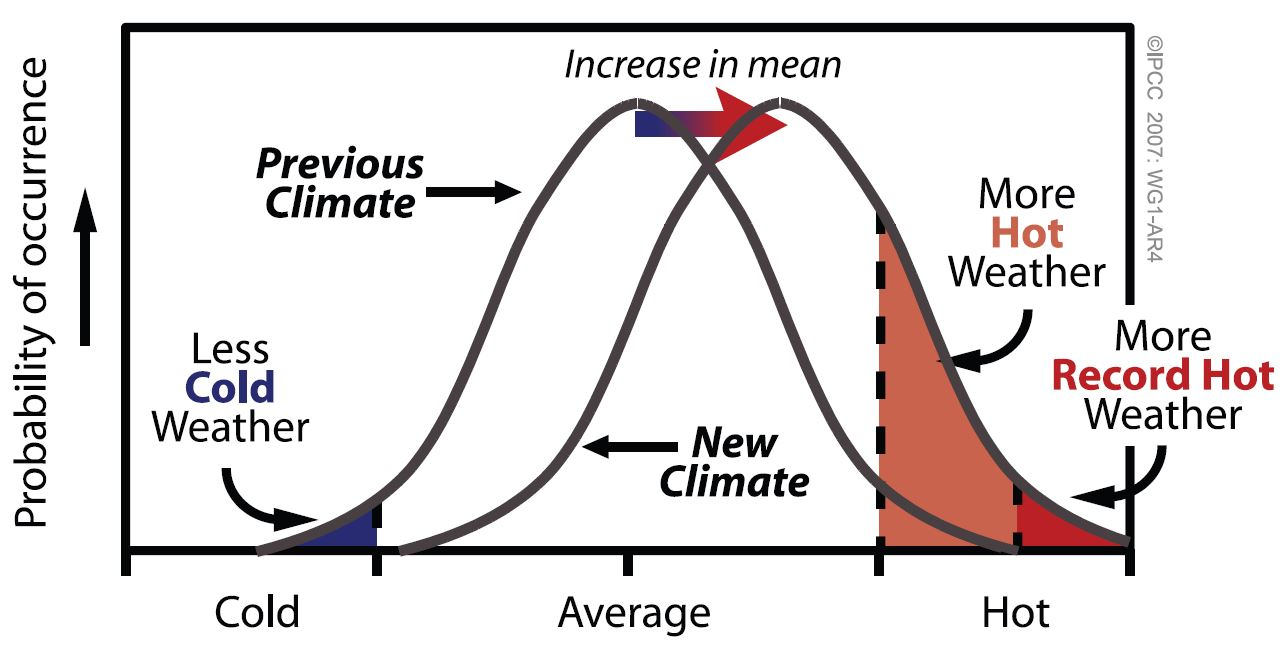
\includegraphics{figs/Fig1.1.jpg}
\caption{\label{fig:fig-1-1}Schematic showing the increase in frequency of extreme
temperatures (shaded light pink) and the magnitude of extreme
temperatures (shaded dark pink), in response to increasing mean
temperature for a normal distribution of temperatures. `extreme' refers
to events that would have been anomalous under the previous probability
distribution. Figure taken directly from \citet{ipcc_climate2007}.}
\end{figure}

\subsection{Range shifts due to climate
change}\label{range-shifts-due-to-climate-change}

Species may track optimal climatic conditions by shifting their range.
This commonly occurs through net population extinctions at the trailing
edge, or net population colonisations at the leading edge
\citep{parmesan_poleward1999}. Dispersal by individuals may also occur
in highly mobile species. Since the predominant effect of climate change
is increasing temperature, many species track temperature by moving to
higher latitudes --- as exemplified in the Arctic, where organisms such
as shrubs and red foxes have expanded polewards
\citep{hersteinsson_interspecific1992, sturm_climate2001}. Others move
to higher altitudes; both latitudinal and altitudinal shifts have been
seen in birds and butterflies of temperate regions
\citep{hill_responses2002, parmesan_poleward1999, thomas_birds1999}.

Until recently, there were very few studies of range shifts due to
climate change in tropical species, with some suggesting that the
response should be less extreme given the slower rates of warming in the
tropics \citep{freeman_rapid2014, ipcc2013}. It is now apparent that
tropical species do shift their ranges to track climate, particularly to
higher elevations \citep{chen_elevation2009, pounds_biological1999}
owing to shallow temperature gradients across latitudes
\citep{colwell_global2008}. In fact, tropical species track climate more
closely than temperate species \citep{freeman_rapid2014}. This effect
could be due to: (1) greater thermal specialisation as a result of
long-term thermal stability in the tropics \citep{freeman_rapid2014};
(2) slower velocity of climate change up mountains
\citep{loarie_velocity2009} meaning it is easier for species to keep
pace; or (3) fewer barriers to dispersal in the tropics, since tropical
biomes have thus far retained a greater proportion of natural habitat
than temperate regions. In any case, even tropical species do not track
climate precisely \citep{chen_elevation2009}.

\subsection{In situ adaptation to climate
change}\label{in-situ-adaptation-to-climate-change}

In situ adaptation encompasses biochemical buffering, gene expression,
phenotypic plasticity, behaviour and genetic adaptation
\citep{peck_organisms2011}. Adaptation is complex and largely
unpredictable; hence it is rarely accounted for in models used to
predict range shifts \citep{peck_organisms2011}. This may be one of the
reasons that species do not move as quickly as predicted.

Modifications in species' phenology represent the vast majority of
documented adaptations to climate change in situ. Many of these examples
come from temperate regions of the Northern hemisphere, where
seasonality is the overarching determinant of species' phenology, and is
itself dramatically altered by climate change
\citep{bradshaw_evolutionary2006}. Specifically, spring has advanced and
the growing season has lengthened. Organism responses include earlier
breeding in animals such as birds and butterflies, earlier arrival of
migratory birds, and earlier flowering in plants
\citep{walther_ecological2002}.

Responses such as physiological plasticity or genetic adaptation feature
much less in the literature on in situ adaptation to climate change.
This may signify a real scarcity of such changes in nature. The
evolution of new forms that enable persistence in the same geographic
range under a changing climate requires a species to become tolerant of
a climatic regime to which it was previously intolerant, which seems
unlikely \citep{parmesan_ecological2006}. One could argue that selective
pressures to evolve increased thermal tolerance would have been
insufficient prior to present-day climate change. However, major
evolution at the species level is not evident in the fossil record
during the Pleistocene glaciation event, even though this comprised
climate change of 5-10 times the magnitude of 20th Century warming
\citep{parmesan_ecological2006}.

While evidence for evolutionary responses to climate change is limited,
this is not to say that evolution has no role to play. Where examples of
such responses do exist, they underlie aforementioned ecological changes
in phenology or dispersal \citep{parmesan_ecological2006}. For example,
Dutch great tits that display greater plasticity in their timing of
reproduction are better able to match egg-laying to food availability --
the peak of which has advanced as a result of climate change -- and thus
achieve greater fitness \citep{nussey_selection2005}. There are also
practical explanations for the lack of documented evolutionary
responses, since these adaptations are less intuitive and harder to
document than ecological responses \citep{oconnor_toward2012}.

The literature discussed above fails to mention one additional and very
significant tool that animals can employ to adapt to climate change --
behaviour. All organisms ordinarily experience a range of temperatures,
and so possess thermoregulatory behaviours that can also be deployed to
mitigate the impacts of climate change. Chamois, for example, move to
higher altitudes and reduce activity when temperature increases
\citep{mason_predicting2014}.

Habitats present a considerable degree of variation in microclimates,
because of variation in microhabitat features
\citep{scheffers_microhabitats2014}, slope and aspect
\citep{suggitt_habitat2011}. Behavioural plasticity allows animals to
move into these microclimates \citep{scheffers_microhabitats2014} and so
track their optimal climate on a local scale. These so-called
``microrefugia'' are utilised by a variety of taxa around the world. In
boreal forests of Finland, moose seek out the cooler microclimates of
forests with higher and denser canopies, in response to high daytime
temperatures \citep{melin_moose2014}. Similarly, in the tropics, possums
choose the coolest tree hollows in which to den
\citep{isaac_microclimate2008}, and herpetofauna of Singapore occupy
microrefugia that not only largely avoid their critical thermal maxima
(CT\textsubscript{max}) -- which is often exceeded in the wider
macroclimate -- but their microrefugia also heat less quickly than the
macroclimate \citep{scheffers_microhabitats2014}.

\section{Influence of land-use
change}\label{influence-of-land-use-change}

The most well-known interaction between climate change and land-use
change is probably that the latter can cause the former, on a global
scale, through the release of GHGs \citep{ipcc2013}. Deforestation
marginally reduces the net radiative forcing that leads to global
climate warming through decreases in surface albedo \citep{ipcc2013}.
Climate change could also cause land-use change, such as through
shifting the areas which are most climatically suited for agriculture
\citep{opdam_climate2004}.

In this review, however, I have focused on how organisms can adaptively
respond to change. The question then becomes: how does land-use change
influence an organism's capacity to respond to climate change? On a
regional scale under wholesale conversion, the answer is relatively
well-discussed. Namely, regional habitat loss creates barriers to
climate-driven range shifts \citep{thomas_protected2012}. Recall that in
response to climate change that has already happened, organisms have not
moved as quickly as expected \citep{chen_elevation2009}, and barriers to
dispersal may contribute to this.

In situ adaptation may allow organisms to persist in habitats from which
they are unable to move, or it may remove the need to move altogether;
in either case, the influence of land-use change on in situ adaptation
to climate change has not been elucidated. Given that many barriers to
dispersal have already been introduced, and this will likely continue
into the future, it is vital to facilitate adaptation to future climate
change within the areas that species already occupy.

Most obviously, wholesale conversion of natural or semi-natural habitat
appears to increase local daytime mean temperature
\citep[e.g.][]{wickham_comparison2012}. Largely, this is caused by an
increase in daily maximum temperature as a result of decreased
interception by overhead vegetation of direct solar radiation
\citep{xu_scale-dependent2004}. The effect is reversed at night when
outgoing long-wave radiation is lost because of reduced interception by
vegetation \citep{xu_scale-dependent2004}. An increase in mean
temperature may exceed an organism's preferred body temperature, and so
potentially lead to sublethal effects \citep{du_plessis_costs2012}, but
increasing maximum temperature generally poses the greater threat to
organisms. Organisms can often acclimate to moderate increases in
average temperatures \citep{peck_animal2009}, but if their critical
thermal maximum is exceeded -- even for a very short amount of time --
this will cause death. Thus, species remaining in habitat after it has
been converted are already likely to be under some amount of thermal
stress, and future climate change may push temperatures beyond the range
that they can tolerate through physiological plasticity.

Any increase in ambient temperature will ultimately increase the
temperature of microclimates, and so potentially decrease their efficacy
as thermal microrefugia for thermally stressed individuals. The extent
to which microclimate utility is compromised depends upon the rate at
which they warm alongside macroclimate warming. There is evidence from
the tropics that this relationship is non-uniform, with microhabitat
temperatures increasing only 0.11--0.66°C for every 1°C in the
macroenvironment \citep{scheffers_microhabitats2014}. Asymmetry in
warming rates will be influenced by factors that act to create the
microclimate, such as the microhabitat
\citep{scheffers_microhabitats2014}, slope, aspect or elevation
\citep{suggitt_habitat2011}. It is possible that microclimates could be
entirely removed as a consequence of microhabitat removal
\citep[e.g.~loss of some bird's nest fern species upon conversion of
forest to oil palm plantation;][]{fayle_effect2009} or extreme
macroclimate warming \citep{caillon_warming2014}.

Wholesale conversion is very likely to impede the ability of persisting
organisms to adapt to future climate change, but then few of the
original species do persist through conversion
\citep[e.g.][]{gibson_primary2011, katovai_understory2012, murphy_meta-analysis2014}
and --- at least in the tropics --- habitat degradation is far more
pervasive. In particular, some 20\% of the humid tropical biome
experienced selective logging from 2000-2005
\citep{asner_contemporary2009}, whilst deforestation affected only 1.4\%
in the same period \citep{hansen_humid2008}. Although the habitat type
broadly remains as `forest', selective logging can be extremely
disruptive. Indeed the term `selective' is somewhat of a misnomer,
meaning that particular species and stems (usually above a minimum trunk
diameter) are targeted \citep{edwards_maintaining2014}. These targets
are typically the largest, oldest trees, the removal of which reduces
canopy height and canopy density
\citep{kumar_effects2005, okuda_effect2003}, and also fragments the
forest canopy and opens up large gaps \citep{edwards_maintaining2014}
that are often invaded by non-tree species, such as climbers and bamboo.
Commercial selective logging also causes collateral damage, particularly
where trees are connected by climbers \citep{schnitzer_recruitment2004},
as well as requiring roads and skid trails that bring further challenges
for wildlife \citep{brodie_correlation2014, laurance_global2014}, and
heavy machinery that result in soil compaction
\citep{putz_reduced-impact2008}.

Since selective logging reduces canopy cover, just as deforestation
does, so it is likely that the thermal regimes of degraded forest will
be similarly altered. Moreover, there is already some indication that
previously identified tropical microrefugia \citep[in this case, leaf
litter and soil;][]{scheffers_microhabitats2014}, are reduced by logging
\citep{saner_reduced2009}. Conversely, ground vegetation --- another
microrefugium \citep{scheffers_microhabitats2014} --- may be favoured by
the release of pioneer species upon the creation of treefall gaps.

The impact of habitat degradation on species' ability to persist under
climate change is likely to be less profound than under wholesale
conversion, simply because the amount of habitat change is less.
However, a greater proportion of species found in undisturbed habitat
remain in degraded habitat than in converted habitat
\citep{edwards_degraded2011}, and it is these species that are of
primary conservation concern. Furthermore, degraded forests now
represent a significant proportion of the humid tropical biome, and are
therefore home to a significant proportion of all tropical forest
species on Earth. The potential for these species to track climate
change through dispersal is limited -- there are barriers, such as
hostile land-use types, as well as a shallow latitudinal temperature
gradient \citep{colwell_global2008} and a potential lack of connected,
higher elevation habitat \citep{scriven_protected2015}. Many tropical
species will need to adapt to climate change within degraded forest, if
they are to persist into the future. Therefore, although we do not yet
fully understand the impact of any land-use change on the ability of
tropical species to adapt in situ to climate change, I argue that we
should first explore the impacts of habitat degradation, as a priority.

\section{Thesis aims and rationale}\label{thesis-aims-and-rationale}

\subsection{Definitions}\label{definitions}

`Microhabitats' are fine-scale (mm to cm) features within a habitat,
including leaf litter, deadwood, tree holes and epiphytes within
rainforest habitats. Each of these features will have its own
`microclimate' which may be different from the macroclimate that acts at
the level of the whole habitat (m to ha). When microhabitat features
offer a more desirable microclimate than the macroclimate, the features
can be referred to as `thermal microrefugia' (`microrefugia'
henceforth).

\subsection{Chapter 2 -- A pantropical analysis of the impacts of forest
degradation and conversion on local
temperature}\label{chapter-2-a-pantropical-analysis-of-the-impacts-of-forest-degradation-and-conversion-on-local-temperature}

SUMMARY

\subsection{Chapter 3 -- A framework for quantifying fine-scale thermal
heterogeneity in the
field}\label{chapter-3-a-framework-for-quantifying-fine-scale-thermal-heterogeneity-in-the-field}

SUMMARY

\subsection{Chapter 4 -- Tropical forests are thermally buffered despite
intensive selective
logging}\label{chapter-4-tropical-forests-are-thermally-buffered-despite-intensive-selective-logging}

SUMMARY

\subsection{Chapter 5 -- The impact of recent forest cover change on
climate connectivity in the
tropics}\label{chapter-5-the-impact-of-recent-forest-cover-change-on-climate-connectivity-in-the-tropics}

SUMMARY

\chapter{A pantropical analysis of the impacts of forest degradation and
conversion on local
temperature}\label{a-pantropical-analysis-of-the-impacts-of-forest-degradation-and-conversion-on-local-temperature}

\begin{figure}[!htb]
\centering
\includegraphics[width=15cm]{pics/Bornean_horned_frog.jpg}
\caption*{Bornean horned frog (\textit{Megophrys nasuta}).}
\end{figure}

\pagebreak

\section{Abstract}\label{abstract-1}

Temperature is a core component of a species' fundamental niche. At the
fine scale over which most organisms experience climate (mm to ha),
temperature depends upon the amount of radiation reaching the Earth's
surface, which is principally governed by vegetation. Tropical regions
have undergone widespread and extreme changes to vegetation,
particularly through the degradation and conversion of rainforests.
Since most terrestrial biodiversity is in the tropics, and many of these
species possess narrow thermal limits, it is important to identify local
thermal impacts of rainforest degradation and conversion. We collected
pantropical, site-level (\textless{} 1 ha) temperature data from the
literature to quantify impacts of land-use change on local temperatures,
and to examine whether this relationship differed above-ground relative
to below-ground and between wet and dry seasons. We found that local
temperature in our sample sites was higher than primary forest in all
human-impacted land-use types (N = 113,894 day-time temperature
measurements from 25 studies). Warming was pronounced following
conversion of forest to agricultural land (minimum +1.6°C, maximum
+13.6°C), but minimal and non-significant when compared to forest
degradation (e.g.~by selective logging; minimum +1°C, maximum +1.1°C).
The effect was buffered below-ground (minimum buffering 0°C, maximum
buffering 11.4°C), whereas seasonality had minimal impact (maximum
buffering 1.9°C). We conclude that forest-dependent species that persist
following conversion of rainforest have experienced substantial local
warming. Deforestation pushes these species closer to their thermal
limits, making it more likely that compounding effects of future
perturbations, such as severe droughts and global warming, will exceed
species' tolerances. By contrast, degraded forests and below-ground
habitats may provide important refugia for thermally-restricted species
in landscapes dominated by agricultural land.

\section{Introduction}\label{introduction}

It is well established that temperature is important in ecology, for
everything from biochemistry, to physiology, to biogeography
\citep{thomas_extinction2004, kearney_potential2009, kingsolver_welltemperatured2009, puurtinen_temperature-dependent2015}.
Temperature is a key explanatory variable in species distribution models
that predict the likely impacts of projected global climate change on
biodiversity \citep[e.g.][]{thomas_extinction2004}. However, the
majority of organisms experience temperature at much finer spatial scale
\citep{gillingham_relative2010, suggitt_habitat2011} than assumed in
species distribution models (often \textgreater{} 100
km\textsuperscript{2}), and at local scales temperature is more
dependent on local factors \citep{suggitt_habitat2011} than on regional
or global atmospheric circulation
\citep{oke_boundary1987, davin_climatic2010, wiens_matching2010, pielke_land2011}.
One such local factor is vegetation cover, which influences temperature
through direct absorption and reflection of incident solar radiation
\citep{oke_boundary1987, murcia_edge1995, snyder_analyzing2004} and
through evapotranspiration, by determining the amount of thermal energy
dissipated through the evaporation of water as opposed to a change in
temperature
\citep{oke_boundary1987, findell_modeled2007, lawrence_effects2015}.

Land-use change can profoundly influence vegetation cover. Current and
future land-use change is concentrated in the tropics, where
\textgreater{} 150 million hectares of forest was converted between 1980
and 2012 \citep{gibbs_tropical2010, hansen_high-resolution2013} and 20\%
of the humid tropical biome was selectively logged from 2000 to 2005
\citep{asner_contemporary2009}. Previous studies, from a range of
disciplines, demonstrate that land-use change in the tropics tends to
increase temperature
\citep{findell_modeled2007, loarie_velocity2009, davin_climatic2010, luskin_microclimate2011, pielke_land2011, ramdani_local2014, lawrence_effects2015}.
This suggests severe consequences for global terrestrial biodiversity,
most of which is found in tropical rainforests
\citep{myers_biodiversity2000} and is thought to be especially sensitive
to temperature change, owing to narrow thermal limits
\citep{deutsch_impacts2008, tewksbury_putting2008, kingsolver_welltemperatured2009}.

Additionally, while absolute warming from global climate change will be
highest at the poles \citep{ipcc2013}, it is the tropics where relative
warming will be greatest, with historically unprecedented temperatures
occurring by 2050 \citep{mora_projected2013}. It is frequently stated
that habitat fragmentation from land-use change will make it
increasingly difficult for tropical species to track climate
\citep{brook_synergies2008, scriven_protected2015}, hampered by the poor
dispersal ability of many tropical species
\citep{van_houtan_dispersal2007} and shallow latitudinal temperature
gradients \citep{colwell_global2008}. However, it is less commonly
discussed that the baseline temperature onto which global climate
predictions are projected might itself be dramatically higher in altered
land-use types \citep{foster_establishing2011, tuff_framework2016}.

To understand current and future consequences for tropical biodiversity
from land-use change and climate change it is vital to understand
thermal change at the scale at which temperature is experienced by
organisms
\citep{wiens_matching2010, gillingham_relative2010, suggitt_habitat2011}.
Prior evidence for local warming in the tropics as a result of land-use
change originates from global General Circulation Models
\citep{findell_modeled2007, davin_climatic2010, pielke_land2011} and
observational studies focused on particular locations, such as Brazil
\citep{loarie_velocity2009}, Malaysia \citep{luskin_microclimate2011}
and Indonesia \citep{ramdani_local2014}. While General Circulation
Models are limited in biological relevance by their coarse spatial
resolution, observational studies are limited in generality by the
site-specificity required to achieve their fine spatial resolution
\citep{li_local2015}. Any studies that utilise meteorological station
data have limited biological relevance because stations are specifically
positioned to minimise the influence of the very same local
characteristics that are important to local biota, such as vegetation
cover, slope and aspect \citep{frenne_weather2016}.

There are several conditions under which local warming due to land-use
change might be ameliorated, which have yet to be explicitly tested. We
hypothesise that low intensity forest degradation, including commercial
selective logging, fragmentation and forest regrowth
\citep{lewis_increasing2015}, will correspond to relatively little net
change in vegetation, and hence a smaller difference in temperature. Any
warming effects of land-use change are likely reversed at night, as
habitats with relatively low vegetation cover will radiate heat back to
the atmosphere more freely
\citep{oke_boundary1987, chen_growing-season1995}. Water availability is
fundamental in determining how much thermal energy can be dissipated
through evaporation, and so we also expect that warming would be less
during the wet season given the high water availability (and more cloudy
weather) relative to dry season, and below-ground relative to
above-ground. In the latter case, even when water availability is very
low, soil buffers external temperature change
\citep{scheffers_microhabitats2014-1} because soil has a higher specific
heat capacity than air, and thus requires a greater change in thermal
energy to achieve the same change in temperature
\citep{oke_boundary1987}.

In the present study, we carry out analyses of published data to test
the effect of land-use change on local temperature across the tropics.
We collected local, in situ temperature data from the literature for
paired sites (\textless{} 1ha) that differed in land-use type.
Categories of land use we studied were primary forest, degraded forest,
plantation, pasture and cropland \citep[\autoref{tab:tab-2-1}; modified
from Extended Data Table 1 in][]{newbold_global2015}. We examine how
land-use change affects day-time temperature at fine-scale spatial
resolution, and we quantify the effects of: (1) forest conversion
compared with forest degradation; (2) below-ground compared to
above-ground; and (3) wet season conditions compared to the dry season.
We focus on day-time temperatures because few studies collected
night-time temperature, although we also separately test how the latter
is impacted by land-use change for the subset of studies able to provide
these data. Recent studies also highlight the importance of climatic
extremes for species' survival
\citep[e.g.][]{deutsch_impacts2008, christidis_role2013}, hence we
conduct additional analyses for those studies that provide these data.

\begin{table}
\begin{center}
\renewcommand{\arraystretch}{1} % reduce space between rows
\setlength{\tabcolsep}{5pt} % reduce space between columns
    \begin{tabular}{ lp{11cm}}
    \toprule 
    \bfseries Land-use type & \bfseries Definition \\ \midrule
    Primary forest  & Forest where any disturbances identified are very minor (e.g. a trail or path)
                      or very limited in the scope of their effect (e.g. hunting of a particular
                      species of limited ecological importance).\\
    Degraded forest & Forest with one or more disturbances ranging from moderate intensity/breadth
                      of impact (e.g. selective logging and bushmeat extraction), to severe
                      intensity/breadth of impact (e.g. regrowth after clear-felling).\\
    Plantation      & Extensively managed or mixed timber, fruit/coffee, oil-palm or rubber
                      plantations.\\
    Cropland        & Farming for herbaceous crops, without presence of livestock. \\
    Pasture         & Farming of livestock.\\
    \bottomrule
    \end{tabular}
\end{center}
\caption{\label{tab:tab-2-1}Land use classification definitions (modified from Extended Data Table 1 in \citet{newbold_global2015}.}
\end{table}

\section{Methods}\label{methods}

\subsection{Literature search}\label{literature-search}

We collated temperature data from peer-reviewed literature using ISI Web
of Knowledge. The search terms were: ``tropic*'' AND (``temperature'' OR
``local climate'') AND (``land use'' OR landuse OR ``land cover'' OR
landcover OR urban* OR city OR cities OR agri* OR arable OR built* OR
metropol* OR deforest* OR forest\emph{) AND (change OR expansion OR
growth OR encroach} OR modif* OR conversion OR convert*). We refined the
search output by including only the following research areas:
``environmental sciences ecology'', ``remote sensing'', ``agriculture'',
``biodiversity conservation'', ``forestry'', ``urban studies''; this
returned 1,372 published studies. Excluding book chapters (21) and
articles that were deemed irrelevant based on the title (298) or
abstract (484) reduced the total to 525 articles. We reviewed each of
these articles manually. Additional unpublished data (two studies) were
also provided by co-authors (P.G., L.K.G.).

\subsection{Selection criteria}\label{selection-criteria}

All data originated from studies with at least two different sites in at
least two different land-use types. Sites were located between 23.44°
North and South, and the natural vegetation type was defined by authors
as forest. Sites were fully contained within the land-use type of
interest and positioned beneath the canopy (where applicable). Within a
single study, sampling methodology was consistent across all sites and
land-use types. Differences between studies, such as soil depth or the
use of radiation shields for dataloggers, were accounted for by the
analytical approach (see `Statistical analysis'). All sites within a
single study differed in elevation by no more than 150 m.

Data collected through remote sensing or from meteorological stations
were excluded, because they are inherently unrepresentative of local
climatic conditions in forested areas. Meteorological stations are
established to strategically avoid the very same local conditions in
which we are primarily interested \citep{frenne_weather2016}. Acceptable
methods of temperature measurement were those taken in situ, using a
thermometer, temperature probe or temperature dataloggers. We included
temperature data reported as an average across multiple spatial
replicates for each land-use type within a study, provided that (1) the
area over which data were averaged and (2) the number of spatial
replicates within this area was consistent across different land-use
types within the study. We set the maximum area over which data could be
averaged as 1 ha, to ensure our study focused on temperature changes at
a fine spatial scale. Aggregated spatial replicates of measurements
within 1 ha were considered as a single site. Where raw data were
provided, a single site comprised the individual point at which
measurements were taken.

We included data reported as an average across multiple temporal
replicates within a study site, provided that (1) the period of time
over which data were averaged and (2) the number of temporal replicates
within this period was within either day or night and was consistent
across different sites within the study. We set the maximum time period
over which data could be averaged as 183 days (half a year), provided
this time period was entirely within either the dry season or the wet
season, as defined by the authors. Aggregated temporal replicates within
a study site were recorded as a single observation. Where raw data
provided more than one measurement per day, we calculated a daily mean
for each study site (between sunrise and sunset only), each of which
represented a distinct observation. If night-time data were available,
we applied the same approach for observations measured between sunset
and sunrise. For those studies providing more than one temperature
observation per day or night, we also calculated temperature minima and
maxima for the time period(s) available (day or night).

\subsection{Data collation}\label{data-collation}

Where possible, temperature data were extracted from text, tables or
graphs in the publication. Data in graphs were extracted using
DigitizeIt \citep[www.digitizeit.de;][]{scheffers_microhabitats2014}. We
also extracted: site coordinates and elevation; site descriptions of
sufficient detail to enable categorisation into land-use types; season
(dry or wet); time of measurements (day or night); and whether
temperature was recorded above- or below-ground. In many cases,
temperature data or methodological information were reported
inadequately or not at all, in which case authors were contacted
directly for information.

In some cases we were unable to retrieve all the required methodological
information, and made estimates. We estimated coordinates from Google
Earth, based on detailed descriptions in the text, and we estimated
elevation from coordinates using a global digital elevation map at 3-arc
second resolution \citep{nasa_srtm2017}. Unless authors had explicitly
stated that data were collected during day or night, we determined this
by comparing the time of data collection to the time of sunrise and
sunset, estimated from the date of collection and the site coordinates
using solar calculations developed by the National Oceanic and
Atmospheric Administration \citep{noaa_solar}, and implemented in R
using custom functions (\url{https://github.com/rasenior/SolarCalc}).
Our main analyses use day-time temperature only because very few studies
considered night-time temperature, though we retained night-time
temperature data where they were available for an additional, simplified
analysis.

We assigned categories of land use based on Extended Data Table 1 in
\citet{newbold_global2015}, which comprise `primary forest, 'degraded
forest' (renamed from `secondary'), `plantation', `pasture' and
`cropland' (\autoref{tab:tab-2-1}). `Urban' could not be included due to
insufficient data.

\subsection{Statistical analysis}\label{statistical-analysis}

Each data point in our main analysis comprised an observation of
day-time temperature in a particular land-use type. We modelled each
temperature observation against land-use type using a linear mixed
effects model, implemented in the lme4 package \citep{bates_fitting2015}
in R \citep{r_core_team_r:2017}. Studies differed substantially in
methodology and location, hence the identity of the study from which
data were taken was included as a random intercept term. Exploratory
plots suggested that the slope of the relationship between land-use type
and temperature, as well as the intercept, varied by study. The decision
to include a random slope of land-use type, with respect to study
identity, was determined using AIC with the full fixed effects structure
\citep{zuur_mixed2009}. Fixed effects were then selected using backward
stepwise model simplification \citep{zuur_mixed2009}, with the following
categorical variables: land-use type (five levels); position relative to
ground level (above- or below-ground); and season (dry or wet season),
as well as pairwise interactions between land-use type and the latter
two variables. We tested interactions using likelihood ratio tests, and
then removed interactions to test main effects independently. For a
subset of studies with suitable data, we used an analogous approach with
only land-use type included as a fixed effect, to model nocturnal
temperature and also temperature minima and maxima (for day-time and
night-time separately).

Model estimates of local temperature are presented relative to the model
estimate for primary forest (above-ground and in the dry season). Both
the position relative to ground level and seasonality interacted with
land-use change to influence local temperature, but for clarity we
discuss each explanatory variable separately. As such, temperature
differences between primary forest and altered land-use types are
averages across all combinations of position and season. The influence
of position on these thermal differences is presented as an average
across seasons, and the influence of seasonality is an average across
positions.

\begin{figure}
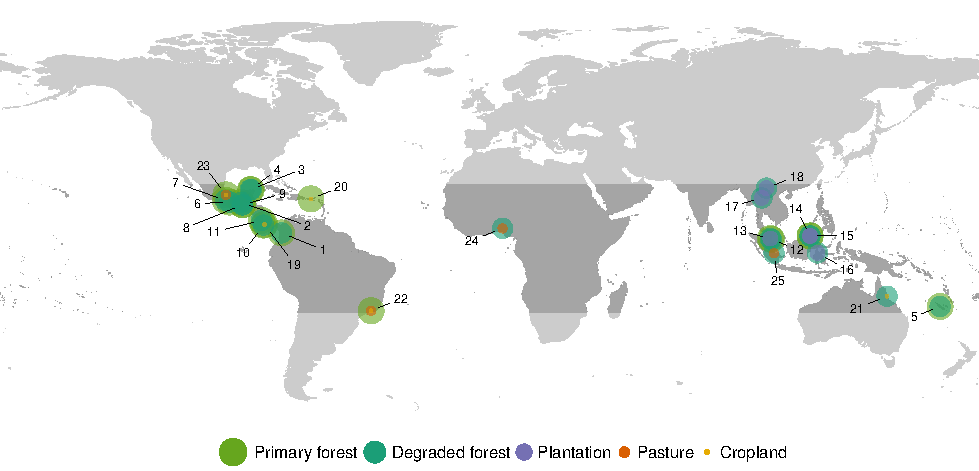
\includegraphics{./output/fig-2-1-1} \caption{Locations of the 25 studies contributing data to the analyses. Point labels correspond to the study number in  Table 1. The shading and size of concentric points corresponds to different land-use types, to indicate the data provided by each study.}\label{fig:fig-2-1}
\end{figure}

\begin{figure}
\centering
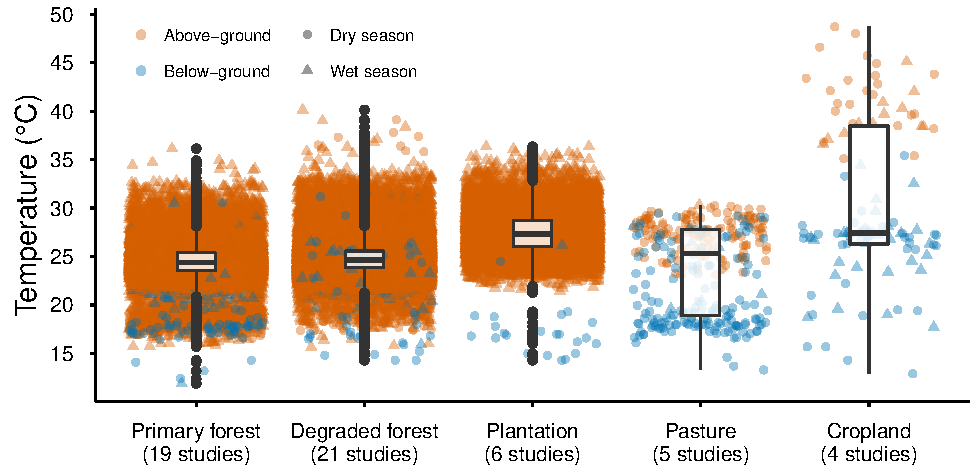
\includegraphics{figs/fig2.2.pdf}
\caption{\label{fig:fig-2-2}Raw day-time temperature against land-use type, across all studies contributing data to the analyses (plotted by study in \autoref{fig:fig-A-1-1}). Point shading indicates temperatures measured above-ground (orange) or below-ground (blue), and different symbols indicate temperatures measured during the dry season (circles) or wet season (triangles).}
\end{figure}

\section{Results}\label{results}

In total, 25 studies met the criteria for inclusion
(\autoref{tab:tab-2-2}). Studies spanned 12 countries, across every
continent within the tropics (\autoref{fig:fig-2-1}), and provided
113,894 observations of day-time temperature (\autoref{fig:fig-2-2} and
\autoref{fig:fig-A-1-1}). Most observations represented either a single
temperature observation within, or mean temperature across, a single day
at the point location where measurements were taken. Six studies
reported temperature at a coarser temporal resolution (mean = 107 days;
minimum = 14 days; maximum = 183 days), and six studies reported
temperature at a coarser spatial resolution (mean = 527
m\textsuperscript{2}; minimum = 64 m\textsuperscript{2}; maximum = 1,000
m\textsuperscript{2}). The maximum elevational difference between sites
within a single study ranged from 0 to 141 m (mean = 33 m), and site
elevation was random with respect to land-use type (LMM,
Χ\textsuperscript{2} = 19.33, df = 14, P \textgreater{} 0.05;
\autoref{fig:fig-A-1-2}). We were also able to obtain 113,459 night-time
temperature observations (including temperature extremes) from 10
studies, plus 113,230 observations of day-time temperature extremes from
11 studies; but none of these data were collected in cropland or
pasture.

In all cases, the final model included a random slope for land-use type
(`LUT') and random intercept with respect to the identity of the study
(`studyID') from which data originated. The final model of day-time
temperature (`temp\_day') included land-use type, position relative to
ground level (`position') and season, as well as pairwise interactions
between land-use type and the latter two fixed effects:

\texttt{lmer(temp\_day\ \textasciitilde{}\ LUT*position\ +\ LUT*season\ +\ (LUT\textbar{}studyID))}

The final models of (1) night-time temperature, and temperature extremes
(minimum and maximum) (2) during the day and (3) during the night, all
had the same model structure, with land-use type as the only fixed
effect:

\texttt{lmer(temp\ \textasciitilde{}\ LUT\ +\ (LUT\textbar{}studyID))}

\begin{sidewaystable}
\renewcommand{\arraystretch}{0.85} % reduce space between rows
\setlength{\tabcolsep}{5pt} % reduce space between columns
\rowcolors{1}{lightgrey}{white}
\begin{tabular}{p{6.5cm}p{2.5cm}p{1.5cm}p{1.5cm}p{1.5cm}p{1.5cm}p{1.5cm}p{1.1cm}p{1.1cm}p{1.13cm}p{1.13cm}}\toprule \hiderowcolors
\bfseries Study & \bfseries Country & \multicolumn{5}{l}{\bfseries Land-use type} & \multicolumn{2}{l}{\bfseries Position} & \multicolumn{2}{l}{\bfseries Season}\\ 
\cmidrule(l{2pt}r{2pt}){3-7} \cmidrule(l{2pt}r{2pt}){8-9} \cmidrule(l{2pt}r{2pt}){10-11}
    & & \bfseries Primary forest & \bfseries Degraded forest & \bfseries Plantation & \bfseries Pasture & \bfseries Cropland & \bfseries Above-ground &
    \bfseries Below-ground & \bfseries Dry season & \bfseries Wet season \\ \midrule \showrowcolors
    1. González del Pliego (Unpublished data) & Colombia      & X & X &   &   &  & X &   & X & \\
    2. González-Di Pierro et al. (2011)       & Mexico        & X & X &   &   &  & X &   &  & X \\
    3. Goode (Unpublished data)               & Mexico        & X & X &   &   &  & X &   &X & X \\
    4. Goode and Allen (2009)                 & Mexico        & X & X &   &   &  & X &   &X & X \\
    5. Ibanez et al. (2013)                   & New Caledonia & X & X &   &   &  & X &   &X & X \\
    6. Lebrija-Trejos et al. (2011)           & Mexico        & X & X &   &   &  & X & X &X & X \\
    7. Negrete-Yankelevich et al. (2007)      & Mexico        & X & X &   &   &  &   & X &  & X \\
    8. Santos (2011)                          & Mexico        & X & X &   &   &  & X & X &  & X \\
    9. Santos and Benítez-Malvido (2012)      & Mexico        & X & X &   &   &  & X & X &  & X \\
    10. Sonnleitner et al. (2009)             & Costa Rica    & X & X &   &   &  & X &   &X &   \\
    11. Wood and Lawrence (2008)              & Costa Rica    & X & X &   &   &  &   & X &  & X \\
    12. Yashiro et al. (2008)                 & Malaysia      & X & X &   &   &  &   & X &X & X \\
    13. Adachi et al. (2006)                  & Malaysia      & X & X & X &   &  &   & X &X &   \\
    14. Hardwick and Orme (2016)              & Malaysia      & X & X & X &   &  & X &   &X & X \\
    15. Hardwick et al. (2015)                & Malaysia      & X & X & X &   &  & X &   &X & X \\
    16. Klein et al. (2002)                   & Indonesia     &   & X & X &   &  & X &   &  & X \\
    17. Wangluk et al. (2013)                 & Thailand      &   & X & X &   &  &   & X &X & X \\
    18. Werner et al. (2006)                  & China         &   & X & X &   &  &   & X &X &   \\
    19. Holl (1999)                           & Costa Rica    & X &   &   & X &  & X & X &X &   \\
    20. Liu and Zou (2002)                    & Puerto Rico   & X &   &   & X &  &   & X &X & X \\
    21. King et al. (1998)                    & Australia     &   & X &   & X &  & X & X &  & X \\
    22. Badejo et al. (2004)                  & Brazil        & X &   &   & X &X &   & X &  & X \\
    23. Campos (2006)                         & Mexico        & X &   &   & X &X &   & X &X & X \\
    24. Badejo (1990)                         & Nigeria       &   & X &   &   &X &   & X &X & X \\
    25. Furukawa et al. (2005)                & Indonesia     &   & X &   &   &X & X & X &X & X \\
\bottomrule
\end{tabular}
\caption{\label{tab:tab-2-2}Summary of the 25 studies contributing data to analyses. Study number corresponds to point labels in \autoref{fig:fig-2-1}. Crosses indicate the land-use types, position(s) relative to ground level and season(s) considered by each study.}
\end{sidewaystable}

\subsection{Effect of land-use change}\label{effect-of-land-use-change}

Altered land-use types were substantially hotter than primary forest
(LMM, Χ\textsuperscript{2} = 29.49, df = 4, P \textless{} 0.001;
\autoref{tab:tab-2-3}; \autoref{fig:fig-2-3}), and the magnitude of the
warming broadly matched the intensity of vegetation change associated
with each land-use type. Thus, degraded forests in our sample were the
most similar to primary forest with an average difference of only
+1.1°C, which was not statistically significant based on 95\% confidence
intervals (\autoref{fig:fig-2-3}). By contrast, converted habitats in
our dataset -- plantation, pasture and cropland -- were, on average,
hotter than primary forest by 2.7°C, 6.2°C and 7.6°C, respectively.
Results were robust to resampling from studies that provided
disproportionate numbers of observations (\autoref{text-A-1-1};
\autoref{fig:fig-A-1-3}).

Night-time temperature, and day-time and night-time temperature
extremes, showed varying results relative to primary forest in the two
altered land-use types for which data were available: degraded forest
and plantation. In all cases, sample sizes were very limited and
confidence intervals were large, hence results should be interpreted
with caution. Night-time temperature in degraded forest and plantation
did not differ from that of primary forest (LMM, Χ\textsuperscript{2} =
2.09, df = 2, P \textgreater{} 0.05; \autoref{fig:fig-A-1-4}), and
neither did night-time minimum temperature (LMM, Χ\textsuperscript{2} =
2.31, df = 2, P \textgreater{} 0.05; \autoref{fig:fig-A-1-5}D). Maximum
night-time temperature was slightly higher overall in degraded forest
and plantation compared to primary forest (LMM, Χ\textsuperscript{2} =
6.35, df = 2, P \textless{} 0.05; \autoref{fig:fig-A-1-5}C), although
pairwise differences were not statistically significant according to
95\% confidence intervals. There was no difference between primary
forest and degraded forest and plantation in terms of day-time maximum
temperature (LMM, Χ\textsuperscript{2} = 4.87, df = 2, P \textgreater{}
0.05; \autoref{fig:fig-A-1-5}A), or day-time minimum temperature (LMM,
Χ\textsuperscript{2} = 4.60, df = 2, P \textgreater{} 0.05;
\autoref{fig:fig-A-1-5}B).

\begin{figure}
\centering
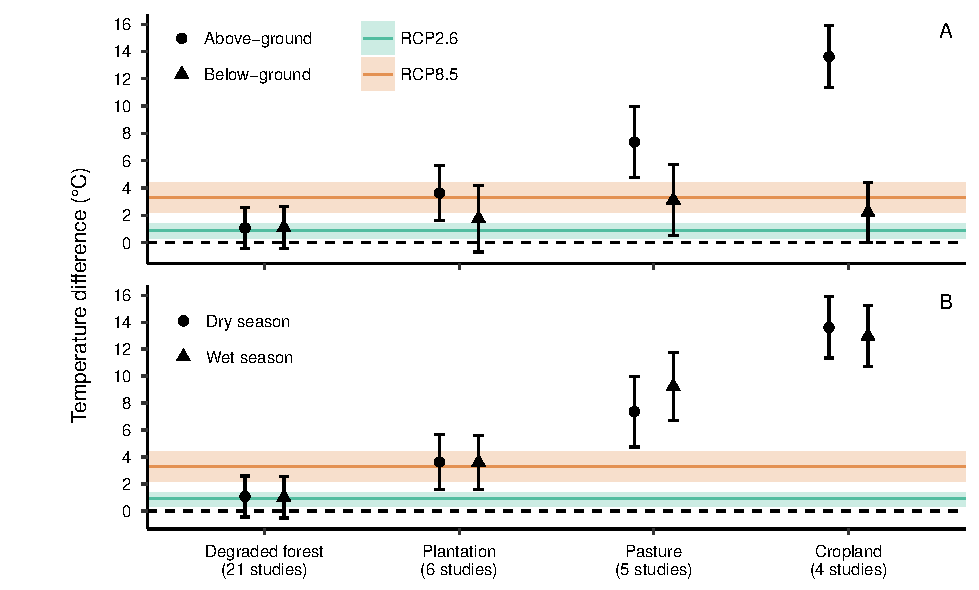
\includegraphics{figs/fig2.3.pdf}
\caption{\label{fig:fig-2-3}Model estimates of local day-time temperature in altered land-use types relative to primary forest (depicted by the black dashed line). In Panel A, different symbols denote position relative to the ground (above-or below-ground), and the season is held at the reference level (dry season). In Panel B, different symbols denote the season (dry or wet), and the position relative to the ground is held at the reference level (above-ground). Error bars are 95\% confidence intervals. Solid lines indicate projected warming in the tropics for the period 2081–2100 compared to the period 1986–2005, as a result of global climate change \citep{ipcc2013}. Shaded bands indicate 5\%–95\% ranges from the distribution of the climate model ensemble. Colors represent the lowest and highest warming scenarios (RCP2.6 and RCP8.5, respectively).}
\end{figure}

\subsection{Above- versus
below-ground}\label{above--versus-below-ground}

The warming effect of land-use change was much stronger above-ground
than below-ground (LMM, Χ\textsuperscript{2} = 1115, df = 4, P
\textless{} 0.001; \autoref{tab:tab-2-3}; \autoref{fig:fig-2-3}A). The
average difference between the local temperature of altered land-use
types and primary forest was greater if measured above-ground rather
than below-ground, by 1.9°C in plantation, 4.3°C in pasture, and 11.4°C
in cropland. In degraded forest, the temperature relative to primary
forest was very similar above- (+1°C) and below-ground (+1.1°C).
Notably, the buffering effect below ground was so great that any
difference between primary forest and impacted land uses was effectively
negated in all land-use types but pasture (based on 95\% confidence
intervals; \autoref{fig:fig-2-3}A).

\subsection{Dry versus wet season}\label{dry-versus-wet-season}

Seasonality had some influence on the relationship between land-use
change and temperature (LMM, Χ\textsuperscript{2} = 14.91, df = 4, P
\textless{} 0.01; \autoref{tab:tab-2-3}; \autoref{fig:fig-2-3}B), but
the direction of the interaction varied by land-use type, and in all
cases the effect size was very small. In degraded forest and plantation,
seasonality had no appreciable effect on temperature relative to primary
forest (dry vs.~wet season: +0.1°C in both degraded forest and
plantation). In contrast, the temperature difference between pasture and
primary forest was 1.9°C greater in the wet versus dry season, while in
cropland the differential was 0.6°C greater in the dry versus wet
season.

\begin{sidewaystable}
\renewcommand{\arraystretch}{1.1} % reduce space between rows
\setlength{\tabcolsep}{5pt} % reduce space between columns
\begin{center}
\begin{tabular}{p{3cm}p{1.3cm}p{1.3cm}p{1.3cm}p{1.3cm}p{1.3cm}p{1.3cm}p{1.3cm}p{1.3cm}p{1.5cm}p{1.3cm}p{1.3cm}p{1.5cm}}\toprule
    \bfseries Land-use type & \bfseries Position & \bfseries Season & \bfseries Temp. vs. PF & \bfseries Lower CI & \bfseries Upper CI & \bfseries LUT mean & \bfseries Position & \bfseries Position mean & \bfseries Position effect (AG-BG) & \bfseries Season & \bfseries Season mean & \bfseries Season effect (dry-wet) \\
    \hline
    Degraded forest & AG & Dry & 1.1 & -0.5 & 2.6 &                     & AG & 1   &                      & Dry & 1.1 &                      \\
                    &    & Wet & 1   & -0.5 & 2.5 &                     &    &     &                      & Wet & 1   &                      \\
                    & BG & Dry & 1.1 & -0.4 & 2.6 &                     & BG & 1.1 &                      &     &     &                      \\
                    &    & Wet & 1   & -0.5 & 2.6 &\multirow{-4}{*}{1.1}&    &     &\multirow{-4}{*}{0.1} &     &     &\multirow{-4}{*}{0.1} \\\rowcolor{lightgrey}
    Plantation      & AG & Dry & 3.6 & 1.6  & 5.6 &                     & AG & 3.6 &                      & Dry & 2.7 &                      \\\rowcolor{lightgrey}
                    &    & Wet & 3.6 & 1.6  & 5.6 &                     &    &     &                      & Wet & 2.6 &                      \\\rowcolor{lightgrey}
                    & BG & Dry & 1.8 & -0.7 & 4.2 &                     & BG & 1.7 &                      &     &     &                      \\\rowcolor{lightgrey}
                    &    & Wet & 1.7 & -0.7 & 4.2 &\multirow{-4}{*}{2.7}&    &     &\multirow{-4}{*}{1.9} &     &     &\multirow{-4}{*}{0.1} \\
    Pasture         & AG & Dry & 7.4 & 4.7  & 10  &                     & AG & 8.3 &                      & Dry & 5.2 &                      \\
                    &    & Wet & 9.2 & 6.7  & 11.8&                     &    &     &                      & Wet & 7.1 &                      \\
                    & BG & Dry & 3.1 & 0.5  & 5.7 &                     & BG & 4   &                      &     &     &                      \\
                    &    & Wet & 5   & 2.4  & 7.5 &\multirow{-4}{*}{6.2}&    &     &\multirow{-4}{*}{4.3} &     &     &\multirow{-4}{*}{-1.9}\\\rowcolor{lightgrey}
    Cropland        & AG & Dry & 13.6& 11.3 & 15.9&                     & AG & 13.3&                      & Dry & 7.9 &                      \\\rowcolor{lightgrey}
                    &    & Wet & 13  & 10.7 & 15.2&                     &    &     &                      & Wet & 7.3 &                      \\\rowcolor{lightgrey}
                    & BG & Dry & 2.2 & 0    & 4.4 &                     & BG & 1.9 &                      &     &     &                      \\\rowcolor{lightgrey}
                    &    & Wet & 1.6 &-0.6  & 3.7 &\multirow{-4}{*}{7.6}&    &     &\multirow{-4}{*}{11.4}&     &     &\multirow{-4}{*}{0.6} \\
\bottomrule
\end{tabular}
\end{center}
\caption{\label{tab:tab-2-3}Model estimates (with 95\% confidence intervals) of local day-time temperature in altered land-use types relative to primary forest (PF), with respect to position relative to ground level and season. 'Position effect' refers to the difference between temperature measured above-ground (AG) versus below-ground (BG), averaged across seasons. 'Season effect' refers to the difference between temperature measured in the dry season versus the wet season, averaged across positions. All figures are quoted in \degree C.}
\end{sidewaystable}

\section{Discussion}\label{discussion}

Our results show that land-use change increases local temperature in the
tropics (\autoref{fig:fig-2-3}). In all conditions where this
relationship was evident, the temperature rise due to land-use change
exceeded that predicted for the tropics by the end of the 21st Century
under the minimum climate warming scenario \citep[+0.9°C in
RCP2.6;][]{ipcc2013}, and frequently also exceeded the maximum warming
scenario \citep[+3.3°C in RCP8.5;][]{ipcc2013}. Previous studies show
that land-use change tends to increase local temperature
\citep[e.g.][]{findell_modeled2007, loarie_velocity2009, davin_climatic2010, luskin_microclimate2011, ramdani_local2014, tuff_framework2016}
but this is the first study, to our knowledge, that demonstrates this
effect across many locations in the tropics at a site-level resolution
(\textless{} 1 ha), considering multiple modes of land-use change
concurrently, and comparing the relationship above- and below-ground and
between wet and dry seasons.

\subsection{Thermal differences between land-use
types}\label{thermal-differences-between-land-use-types}

Human-impacted land-use types are likely hotter than intact primary
forest because of changes in evapotranspiration and the amount of solar
radiation reaching the Earth's surface
\citep{oke_boundary1987, findell_modeled2007, davin_climatic2010}.
Degradation and deforestation cause a lowering and thinning of the
canopy, and reduction in rooting depth, leaf area index and surface
roughness, all of which reduce evapotranspiration
\citep{okuda_effect2003, snyder_analyzing2004, kumar_effects2005, findell_modeled2007, davin_climatic2010, hardwick_relationship2015},
and thereby increase temperature
\citep{oke_boundary1987, foley_global2005}. Changes to canopy
architecture and a reduction in the number of sub-canopy vegetation
strata also cause warming by increasing the amount of solar radiation
reaching the ground \citep{oke_boundary1987, murcia_edge1995}. Our land
use categories encompass a spectrum of vegetation change, from
relatively little change in degraded forests (where some trees and a
closed canopy are maintained) to maximal change in pasture and cropland
(where trees are replaced with herbaceous plants). Accordingly,
degradation had the smallest average effect (+1.1°C), followed by
plantation (+2.7°C), and then pasture (+6.2°C) and cropland (+7.6°C). We
expected that the same mechanisms underlying the warming effect of
land-use change would also result in increased day-time temperature
extremes and decreased night-time temperatures in altered land-use
types, relative to primary forest
\citep{oke_boundary1987, chen_growing-season1995}. Unfortunately, the
data available were very limited, including only three of the five
land-use types (primary forest, degraded forest and plantation), and
resulting in extremely large confidence intervals
(\autoref{fig:fig-A-1-3} and S4). We urge caution when interpreting our
results, which suggested either no effect or an extremely weak effect of
land-use change on temperature extremes and night-time temperature;
clearly more data are needed to reliably test these relationships.

\subsection{Interaction with position relative to ground level and
seasonality}\label{interaction-with-position-relative-to-ground-level-and-seasonality}

We found that local warming effects of tropical land-use change are
negated below-ground, despite the strength of the relationship
above-ground (\autoref{tab:tab-2-3}; \autoref{fig:fig-2-3}A). This can
largely be attributed to the higher specific heat capacity of soil
compared to air \citep{oke_boundary1987}. Greater availability of water
may also play a role, permitting thermal energy to be dissipated through
the evaporation of water rather than increasing temperature
\citep{oke_boundary1987, davin_climatic2010, christidis_role2013}. We
expected the latter effect to result in increased buffering during the
wet season \citep[cf.][]{findell_modeled2007, davin_climatic2010}, but
instead we found that seasonality had a very limited influence on
temperature relative to primary forest (\autoref{tab:tab-2-3};
\autoref{fig:fig-2-3}B). The strongest influence was in pasture, where
the effect of land-use change was greater in the wet season. Potentially
longer grass in pasture in the wet season could decrease albedo compared
to pale exposed soil in the dry season, while the same pattern could be
avoided in cropland through dry season irrigation. That said, pasture
and cropland had the least data of all land-use types, and we advise
that these results be interpreted with caution.

\subsection{Implications for
biodiversity}\label{implications-for-biodiversity}

For tropical biodiversity, there are several key implications of our
findings. Firstly, forest species persisting through forest conversion
have already experienced thermal change similar, if not greater, in
magnitude to that predicted by global climate change \citep{ipcc2013}.
Historically the tropics have experienced relatively stable climatic
conditions \citep{mora_projected2013} and tropical species possess
narrow thermal niches, with many already occupying the upper bounds of
that niche
\citep{deutsch_impacts2008, tewksbury_putting2008, freeman_rapid2014, sunday_thermal-safety2014}.
Dispersal towards more favourable climatic conditions is limited by low
dispersal ability \citep{van_houtan_dispersal2007}, a scarcity of
suitable destinations \citep{colwell_global2008}, and the necessity to
pass through an increasingly hostile land-use matrix to reach target
habitat
\citep{thomas_extinction2004, brook_synergies2008, scriven_protected2015}.
There is already some evidence that higher temperatures in the tropics
are associated with lower species abundance \citep[e.g.~for
arthropods:][]{foster_establishing2011}, and there are also fitness
costs associated with long-term persistence in suboptimal climatic
conditions \citep{du_plessis_costs2012, gunderson_conceptual2016}.
Without any further temperature change some species persisting in
converted environments may already be committed to extinction,
particularly species that are unable to utilise microhabitats with
favourable microclimates
\citep{scheffers_microhabitats2014-1, gonzalez_del_pliego_thermally2016}.
Under predicted climate change, increasing average temperature and the
increasing frequency and intensity of droughts
\citep{chou_changes2012, ipcc2013} will likely push many species beyond
their upper thermal limits, especially in heavily degraded or converted
habitats.

That said, we find several circumstances where warming through land-use
change is mitigated. Degraded forests were not significantly hotter than
primary forests (according to 95\% confidence intervals;
\autoref{fig:fig-2-3}). This is encouraging because degraded forests are
likely to become the most widespread land-use type in future
\citep{hurtt_harmonization2011}, and many studies have demonstrated
their capacity to retain species of conservation concern
\citep{edwards_degraded2011, gibson_primary2011, putz_sustaining2012, edwards_maintaining2014}.
For all altered land-use types, the warming effect was limited
below-ground, highlighting a crucial thermal refuge for species that are
able to occupy the soil, and suggesting that above-ground microhabitats,
such as deadwood and epiphytes, might fulfil a similar role
\citep{scheffers_microhabitats2014-1, gonzalez_del_pliego_thermally2016}.
Thermal refugia may not be a permanent solution for avoiding climate
change, and sensitive species may find that even relatively cold
microhabitats are still too hot (e.g.~below-ground in pasture was 4°C
warmer than primary forest; \autoref{tab:tab-2-3};
\autoref{fig:fig-2-3}), but refugia could at least provide species with
more time to respond to suboptimal climatic conditions
\citep{hannah_fine-grain2014}.

\subsection{Caveats and knowledge
gaps}\label{caveats-and-knowledge-gaps}

By collating site-level data reported from the literature, we were able
to achieve high geographical coverage and fine spatial resolution that
is lacking in previous studies, but this technique is biased by the
availability of data towards particular regions and land-use types
(\autoref{fig:fig-2-1}), and relies heavily on substituting space for
time, which can misrepresent anthropogenic impacts
\citep{franca_space-for-time2016}. In particular, there was only one
study located in Africa, and Southeast Asian studies provided all of the
plantation data and no cropland data. Future research should seek to
explicitly consider how tropical land-use change affects: vegetation
structure \citep[e.g.~using Leaf Area Index
cf.][]{hardwick_relationship2015}, relative humidity
\citep{luskin_microclimate2011, ewers_fragmentation2013}, nocturnal
climatic conditions
\citep{chen_growing-season1995, dubreuil_impact2011}, extremes of
temperature \citep{christidis_role2013}, and rates of temperature change
\citep{scheffers_microhabitats2014-1}; preferably at a range of
spatiotemporal scales \citep{wiens_matching2010} and with a standardised
methodology to simplify comparisons across studies.

\subsection{Conclusions}\label{conclusions}

Our study confirms that tropical land-use change leads to warming at a
local scale (\textless{} 1 ha) across the tropics, of a magnitude
comparable to that predicted from global climate change. We find
pantropical evidence that the effects of land-use change on temperature
are ameliorated below-ground, and absent in degraded forests. Many
studies collect site-level climate data, and through sharing of these
data and collaboration between scientific disciplines, there is much
that can be done to integrate theoretical and empirical understanding of
the processes that govern climate at different scales. This will greatly
advance our knowledge of potential synergies between two of the greatest
drivers of biodiversity loss -- land-use change and climate change --
and highlight mitigating factors, such as thermal microrefugia, which
could be a pragmatic focus for conservation management.

\section{Data and R code}\label{data-and-r-code}

The collated dataset can be found on Dryad
(\url{doi:10.5061/dryad.g4000}). Note that in many cases these data were
aggregated for analyses. For finer resolution data please refer to the
original data sources. R functions used to estimate time of sunset and
sunrise can be downloaded from GitHub
(\url{https://github.com/rasenior/SolarCalc}).

\chapter{A framework for quantifying fine-scale thermal heterogeneity in
the
field}\label{a-framework-for-quantifying-fine-scale-thermal-heterogeneity-in-the-field}

\begin{figure}[!htb]
\centering
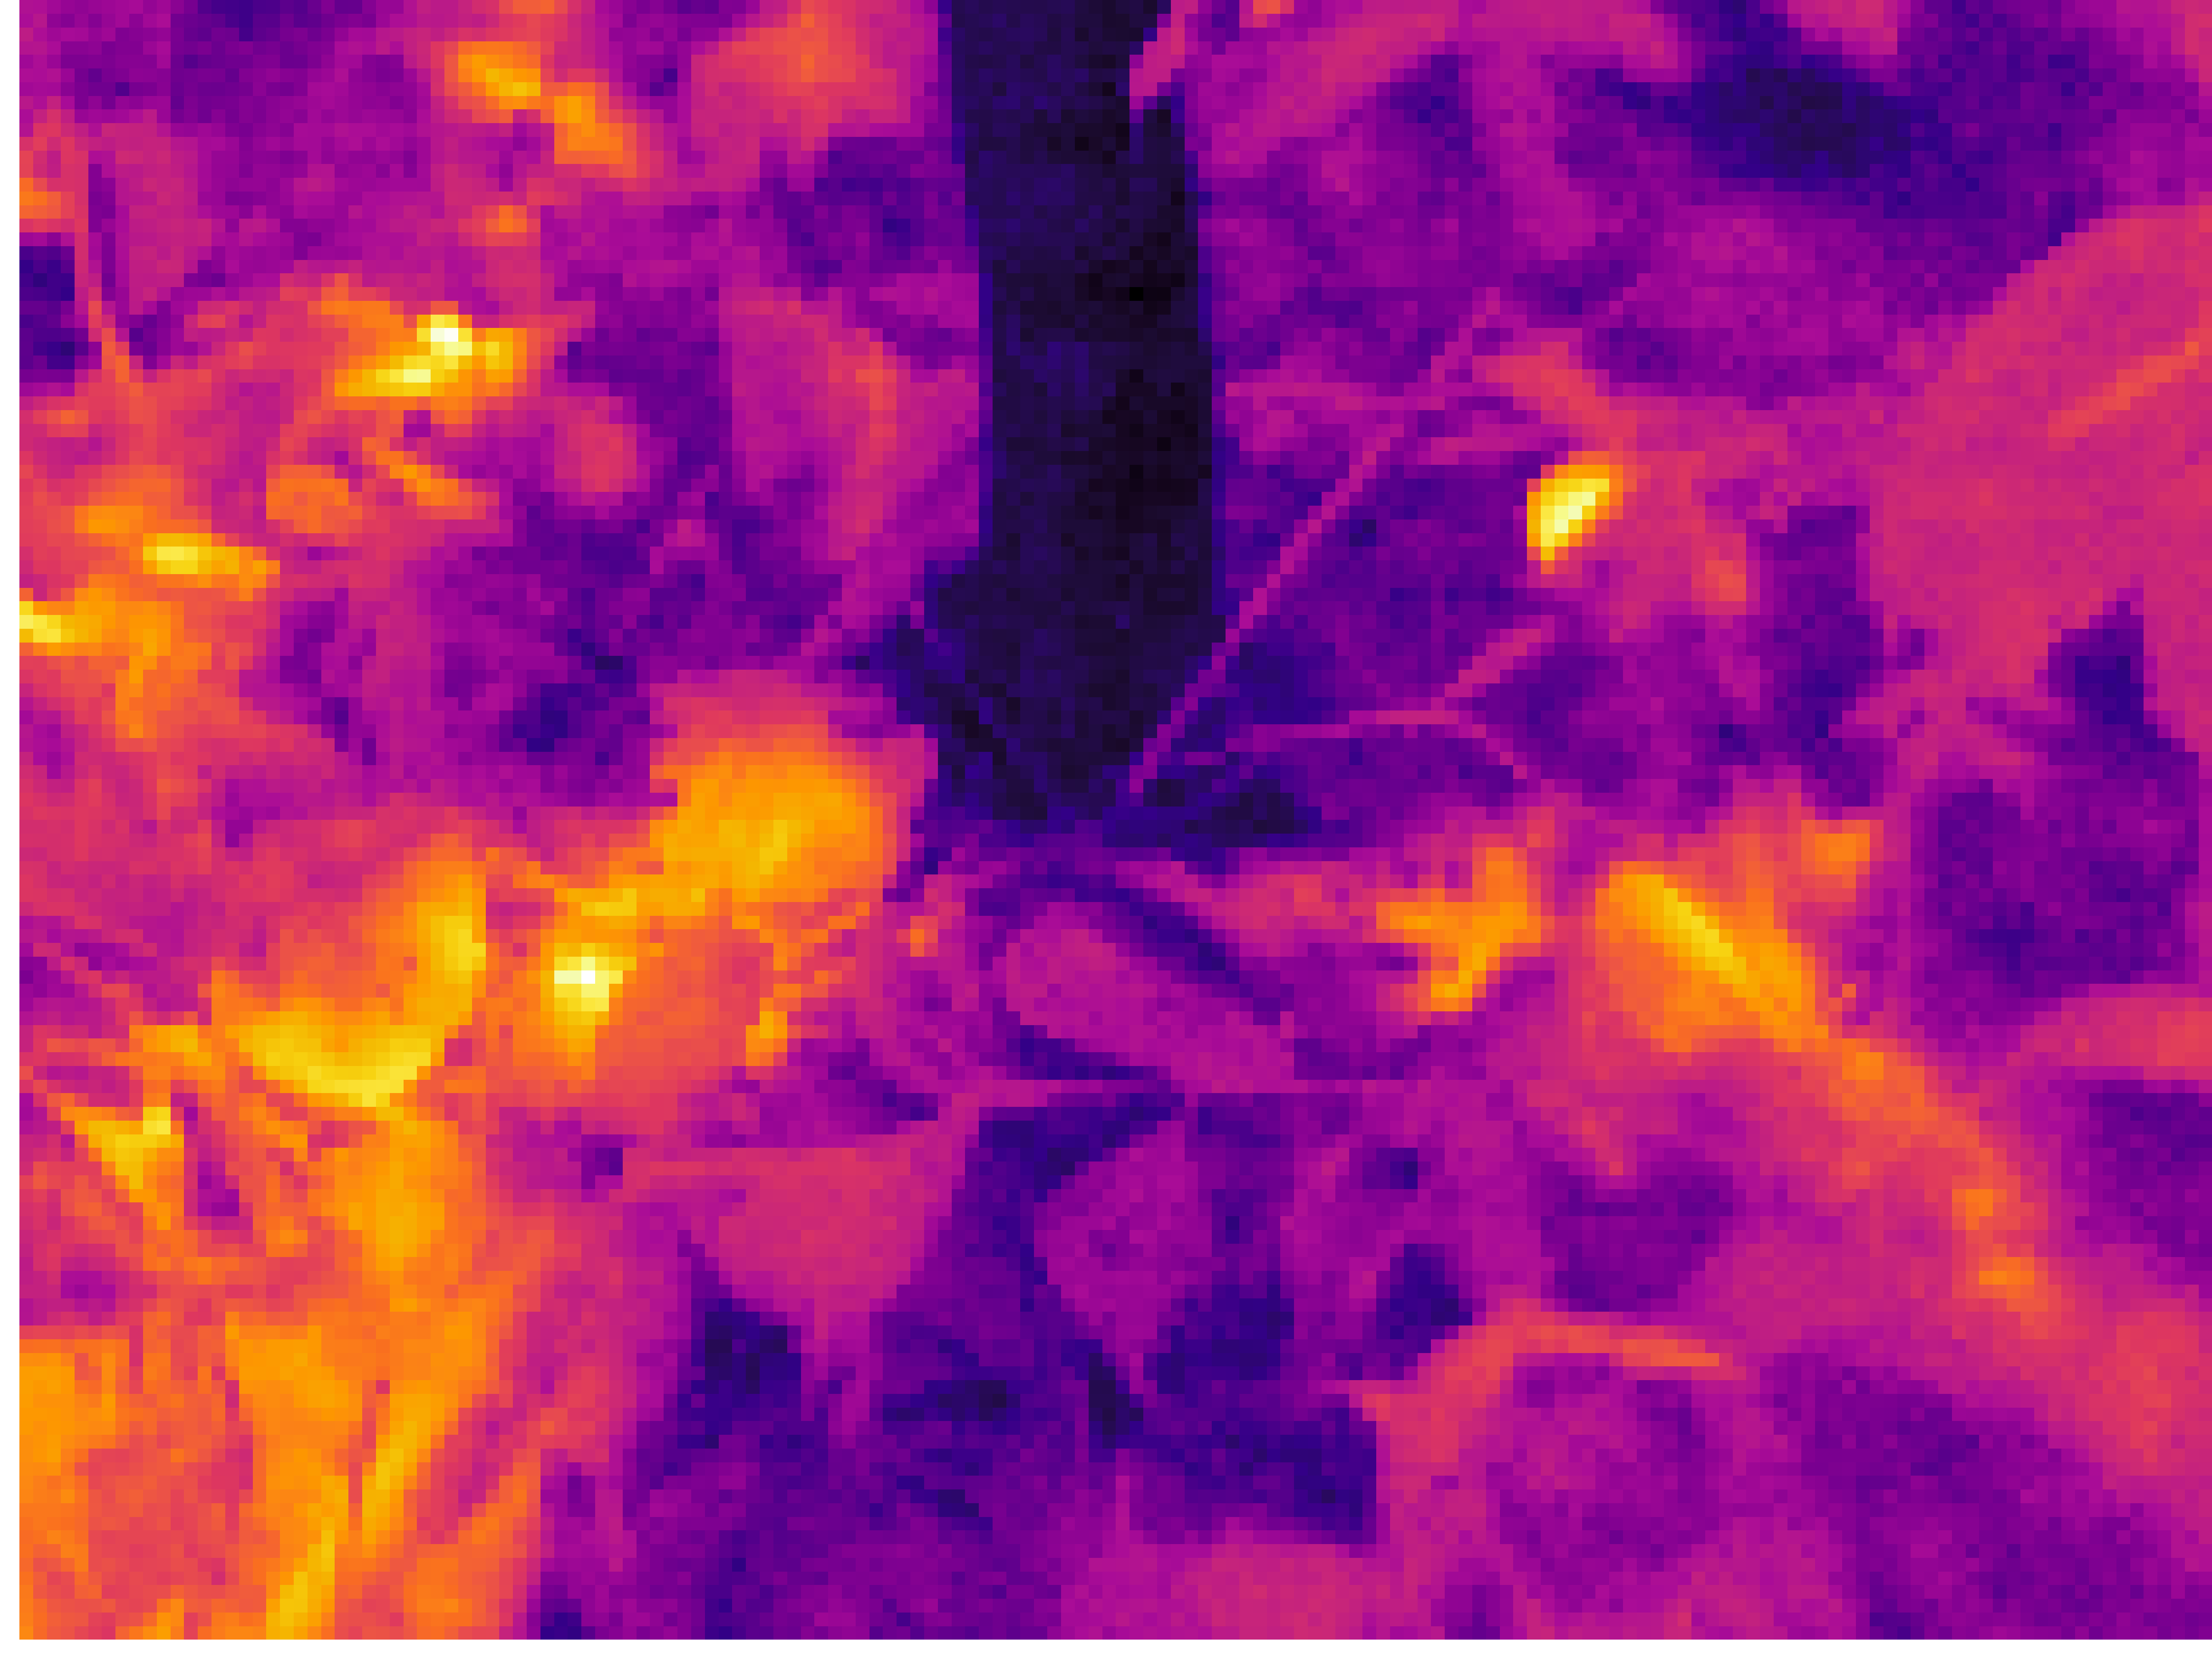
\includegraphics[width=15cm]{pics/Themal-image1.png}
\caption*{Thermal image of rainforest floor.}
\end{figure}

\pagebreak

\chapter{Tropical forests are thermally buffered despite intensive
selective
logging}\label{tropical-forests-are-thermally-buffered-despite-intensive-selective-logging}

\begin{figure}[!htb]
\centering
\includegraphics[width=15cm]{pics/Bornean_tree_hole_frog.jpg}
\caption*{Bornean tree hole frog (\textit{Metaphrynella sundana}).}
\end{figure}

\pagebreak

\section{Abstract}\label{abstract-2}

Tropical rainforests are subject to extensive degradation by commercial
selective logging. Despite pervasive changes to forest structure,
selectively logged forests represent vital refugia for global
biodiversity. The ability of these forests to buffer
temperature-sensitive species from climate warming will be an important
determinant of their future conservation value, although this topic
remains largely unexplored. Thermal buffering potential is broadly
determined by: (1) the difference between the `macroclimate' (climate at
a local scale, m to ha) and the `microclimate' (climate at a fine-scale,
mm to m, that is distinct from the macroclimate); (2) thermal stability
of microclimates (e.g.~variation in daily temperatures); and (3) the
availability of microclimates to organisms. We compared these metrics in
undisturbed primary forest and intensively logged forest on Borneo,
using thermal images to capture cool microclimates on the surface of the
forest floor, and information from dataloggers placed inside deadwood,
tree holes and leaf litter. Although major differences in forest
structure remained 9-12 years after repeated selective logging, we found
that logging activity had very little effect on thermal buffering, in
terms of macroclimate and microclimate temperatures, and the overall
availability of microclimates. For 1°C warming in the macroclimate,
temperature inside deadwood, tree holes and leaf litter warmed slightly
more in primary forest than in logged forest, but the effect amounted to
less than 0.1°C difference between forest types. We therefore conclude
that selectively logged forests are similar to primary forests in their
potential for thermal buffering, and subsequent ability to retain
temperature-sensitive species under climate change. Selectively logged
forests can play a crucial role in the long-term maintenance of global
biodiversity.

\section{Introduction}\label{introduction-1}

Land-use change is a profound threat to Earth's terrestrial biodiversity
\citep{sala_global2000, maxwell_biodiversity:2016}. Most of this
biodiversity is found in tropical regions \citep{jenkins_global2013},
where rates of deforestation and forest degradation are among the
highest globally \citep{hansen_high-resolution2013}. The detrimental
impacts of deforestation on tropical biodiversity are well known
\citep{gibson_primary2011, barlow_anthropogenic2016}; however, tropical
forest degradation via commercial selective logging is 20 times more
widespread than on-going conversion
\citep{hansen_humid2008, asner_contemporary2009}, making it important to
understand the value of these disturbed forests for biodiversity.
Selectively logged forests constitute a large and effective refuge for
species of conservation concern that cannot survive in deforested land
\citep{edwards_degraded2011, gibson_primary2011, edwards_biodiversity2013}.
Protecting selectively logged forests may be a cost effective way to
retain tropical biodiversity \citep{edwards_maintaining2014}, but this
is heavily contingent on the assumption that these forests will maintain
their current conservation value into the future.

Several factors may influence the value of selectively logged forests
for biodiversity in the long-term, and a key consideration is the
interaction of multiple drivers of biodiversity loss
\citep{brook_synergies2008, mantyka-pringle_interactions2012, sirami_impacts2017}.
The impacts of climate change are particularly important, and
increasingly so as this century progresses
\citep{sala_global2000, chou_increase2013, ipcc2013}. Novel
(non-analogous) climatic conditions are predicted to appear first in the
tropics \citep{mora_projected2013}, where many species have narrow
thermal limits
\citep{deutsch_impacts2008, tewksbury_putting2008, khaliq_global2014}
and where there is limited dispersal potential owing to poor dispersal
ability of many species \citep{van_houtan_dispersal2007}. This
vulnerability of tropical species is compounded by an absence of target
habitats containing analogous climates \citep{colwell_global2008}, and
widespread deforestation creating a hostile matrix through which
dispersal must occur \citep{brook_synergies2008, scriven_protected2015}.
The ability of tropical species to withstand climate change, and so
avoid extinction, is likely to be highly dependent on their ability to
adapt \emph{in situ} within existing forest areas. The extent to which
species persistence can be facilitated within selectively logged forests
will, therefore, greatly influence the conservation value of these
habitats.

In primary forests and secondary forests re-growing on abandoned
farmland, previous studies found that organisms -- particularly
ectotherms -- avoid suboptimal temperatures in the wider `macroclimate'
(climate at a spatial scale of m to ha) by moving locally into
`microclimates': climate at a fine-scale, mm to m, that is distinct from
the macroclimate
\citep{scheffers_microhabitats2014-1, scheffers_microhabitats2014, gonzalez_del_pliego_thermally2016}.
Climate at this fine-scale is more relevant for the majority of
terrestrial biodiversity, which primarily consists of small-bodied
ectotherms
\citep{suggitt_habitat2011, potter_microclimatic2013, nadeau_coarse2017}.
Indeed, the vast proportion of terrestrial species are small in size,
flat in shape, or thermoregulate via contact with vegetation, and so it
is important to consider microclimates close to, and including, the
surfaces on which these species live
\citep{kaspari_thermal2015, scheffers_extreme2017}.

The most informative fine-scale temperature data are derived from point
measurements that are highly replicated in both space and time, and
demonstrate that loss of vegetation cover causes local daytime warming
\citep{senior_pantropical2017, ewers_fragmentation2013, hardwick_relationship2015, gonzalez_del_pliego_thermally2016}.
Selective logging affects vegetation by lowering and thinning the
canopy, reducing leaf area index
\citep{hardwick_relationship2015, ewers_logging2015} and the number of
vegetation strata, and creating large forest gaps
\citep{okuda_effect2003, kumar_effects2005}. As such, the understorey of
logged forests likely receives a greater amount of solar radiation,
partitioned increasingly as direct rather than diffuse radiation
\citep{oke_boundary1987}, although these impacts diminish rapidly as
selectively logged forests recover \citep{asner_canopy2004}. The most
tangible impact on the local climate could be an overall increase in the
day-time temperature of logged forests, increasing the necessity for
thermal buffering. Simultaneously, the potential for thermal buffering
may be compromised if forest structural changes also influence the
temperature and distribution of cool microclimates, particularly if
their temperature becomes more similar to that of the wider macroclimate
\citep[e.g.][]{caillon_warming2014}, or there are simply fewer cool
microclimates available overall. Conversely, enhanced air-mixing in more
open logged forests might create cooler and less variable microclimates.
Previous evidence suggests that the availability of cool `microhabitats'
\citep[localised environments within which cool microclimates are
contained;][]{scheffers_microhabitats2014-1, gonzalez_del_pliego_thermally2016, shi_framework2016}
can be reduced \citep[e.g., leaf litter;][]{saner_reduced2009} or
increased \citep[e.g., deadwood;][]{carlson_deadwood2017} by selective
logging, implying that forest quality alters thermal environments.

A key novel question that we address in this paper is whether vegetation
changes following commercial selective logging reduce the potential for
thermal buffering. We focused on cool microclimates in the understorey
only (climate at mm to m scale that is cooler than the macroclimate and
located within \textasciitilde{}2 m of the forest floor). Microclimates
on the surface of the forest floor were captured by a thermal camera,
while dataloggers were used to capture microclimates within cool
understorey microhabitats: leaf litter, tree holes and deadwood
\citep{scheffers_microhabitats2014-1, scheffers_microhabitats2014, gonzalez_del_pliego_thermally2016}.
We determined thermal buffering potential according to: (1) the
microclimate temperature relative to that of the macroclimate; (2) the
daily variation in microclimate temperature; and (3) the availability of
microclimates in space. The first two are roughly measures of
microclimate `quality' -- they examine how effectively an organism will
be buffered from macroclimate warming, assuming it moves into the
microclimate. The third captures the likelihood that organisms can
locate and move into suitable microclimates, according to the
occurrence, distribution and thermal diversity of microclimates within
the habitat \citep{sears_world2011, caillon_warming2014}. We predicted
that logged forests would be structurally distinct from primary forest,
and we tested the hypothesis that this would lead to reduced thermal
buffering potential and, subsequently, impaired ability of
temperature-sensitive species to respond \emph{in situ} to excessively
high temperatures in the wider macroclimate.

\section{Materials and Methods}\label{materials-and-methods}

\subsection{Study area}\label{study-area}

Sampling took place in in an extensive area of contiguous forest in
Sabah (Malaysian Borneo; Fig. 1a). This area represents over 10,000
km\textsuperscript{2} of lowland dipterocarp forest, comprising
production forest and areas of undisturbed protected forest
\citep{reynolds_changes2011}. In this study, we sampled sites in forest
that had been commercially selectively logged twice (Ulu Segama-Malua
Forest Reserve, 4°57'42.8''N, 117°56'51.7''E). The area was first logged
from 1987-1991, using tractors and high-lead extraction techniques to
harvest commercial trees (those in the family Dipterocarpaceae) with
stems \textgreater{} 0.6 m diameter at breast height (D.B.H.), and
yielding \textasciitilde{}113 m\textsuperscript{3} of timber per hectare
\citep{fisher_cost-effective2011, edwards_selective-logging2014}.
Between 2001 and 2007, the area was re-logged and the minimum harvested
tree diameter reduced to \textgreater{} 0.4 m D.B.H., yielding an
additional 31 m\textsuperscript{3}/ha of timber
\citep{fisher_cost-effective2011}. Thus, we sampled sites that had been
heavily disturbed about 10 years prior to the study, at which point 67\%
of the forest had an average density of \textless{} 10 trees per hectare
with a D.B.H. greater than 40 cm \citep{reynolds_changes2011}. The area
has been recovering naturally since logging operations ceased. Control
sites were located in undisturbed, protected primary forest (Danum
Valley Conservation Area; 4°57'45.2''N, 117°48'10.4''E).

\begin{figure}

{\centering 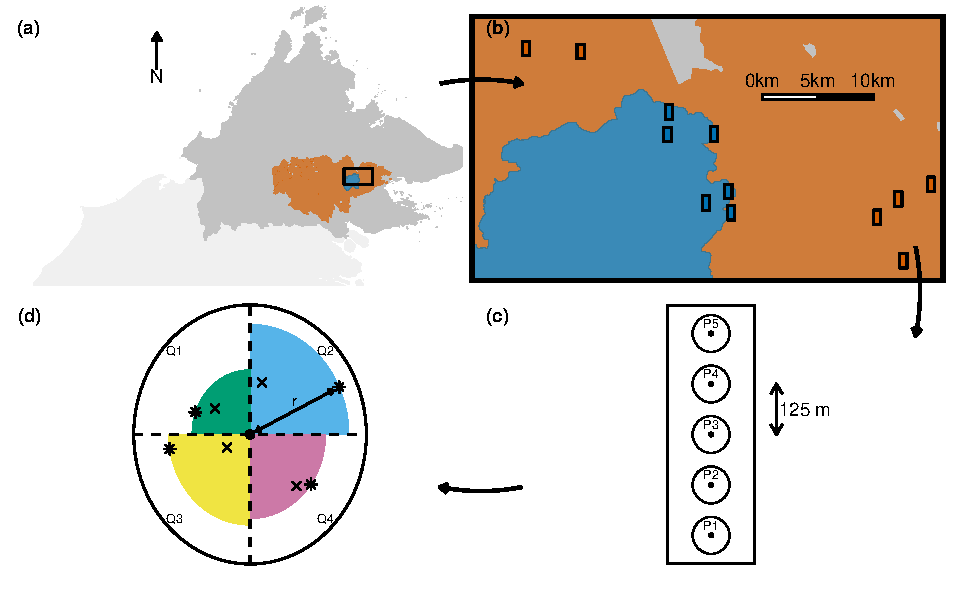
\includegraphics{./output/fig-4-1-1} 

}

\caption{Study location in Malaysian Borneo (a), and distribution of sites (b): six sites in primary forest (blue) and six sites in logged forest (orange). Each site comprised five plots along an existing transect, with plot centres separated by 125 m (c). Tree and sapling stand basal area was calculated from the distance to and circumference of the nearest two trees and saplings in each of four quadrants centred on the plot centre (d; see Supplementary Text S1 for more details). Curved arrows indicate the direction of magnification, from panels a-d.}\label{fig:fig-4-1}
\end{figure}

\subsection{Sampling design}\label{sampling-design}

We sampled twelve sites, six in twice-logged forest and six in primary
forest, along existing transects \citep[Fig.
1b;][]{edwards_degraded2011, edwards_selective-logging2014}. Sites were
more than 2 km apart, and at least 100 m from forest edges. Within each
site, we established five plots 50 m in diameter, with plot centres
spaced at 125 m intervals along the transect (Fig. 1c; 60 plots in
total). Fieldwork was conducted from April to July 2015, during the
severe El Niño-Southern Oscillation (ENSO) event of 2015-2016
\citep{noaa2015} when mean daily temperature was 2.26°C higher and mean
daily rainfall was 2.09 mm lower than the 5-year average (across April
to July for the years 2007 to 2011; data from weather station at Danum
Valley Field Centre).

\subsubsection*{Forest structure}\label{forest-structure}
\addcontentsline{toc}{subsubsection}{Forest structure}

To quantify the level of disturbance to the forest from selective
logging, we used an established methodology for assessing forest
structure in each plot \citep{hamer_ecology2003, lucey_spillover2012}.
The variables we measured were: the stand basal area
(m\textsuperscript{2}/ha) of mature trees (circumference \textgreater{}
0.6 m) and saplings (circumference 0.1-0.6 m), based on the distance to
and circumference at breast height of the two nearest trees and saplings
in each of four quadrants centred on the plot centre (Fig. 1d); the
coefficient of variation for the basal area of trees and of saplings;
the proportion of mature trees that were dipterocarps (indicative of
mature, complex forest); percentage canopy cover; and visual estimates
of percentage vegetation cover at ground (1.5 m above ground),
understorey (15 m above ground) and canopy (the main stratum of leaf
cover \textgreater{} 15 m above ground) height. For full methodological
details see Supplementary Text S1.

\subsubsection*{Quantifying surface
microclimates}\label{quantifying-surface-microclimates}
\addcontentsline{toc}{subsubsection}{Quantifying surface microclimates}

Fine-scale surface temperature of the forest floor is particularly
relevant for small-bodied, surface-dwelling organisms, such as many
insect and reptile species. We measured surface temperature within each
plot using an infrared camera (FLIR Systems, model E40). Macroclimate
temperature was defined as the air temperature at 1.5 m above-ground,
measured using a whirling hygrometer. Each site was visited on two days,
and each plot within the site was sampled five times each day between
05:00 hrs to 14:30 hrs. During each sample of any given plot, the
observer stood at the centre of the plot, took a single hygrometer
reading and then, holding the camera at breast height and pointing 45°
downwards (relative to the ground), took a photo in four orthogonal
directions \citep{scheffers_extreme2017}. Each thermal image comprised
19200 distinct observations of surface temperature (one per pixel), and
covered a surface area of approximately 1 m\textsuperscript{2}. In
total, we recorded 2400 thermal images (4 images per plot x 5 repeats x
2 site visits x 60 plots).

For all subsequent analyses, a unique data point comprised thermal
information from the four photographs taken each time a plot was
sampled: 76800 observations of surface temperature measurements for each
plot (i.e.~combining 19200 observations from the four photos taken in
each orthogonal direction). For details of thermal image data extraction
and processing see Supplementary Text S2. The temperature of cool
surface microclimates was defined as the 5\textsuperscript{th}
percentile (i.e.~coolest) across all 76800 pixels. For some organisms,
the efficacy of thermal buffering also depends on the thermal stability
of microclimates \citep{shi_framework2016}. We calculated daily
variation in surface microclimate temperature as the difference between
the minimum and maximum microclimate temperature, for each day and for
each plot.

To identify spatially-explicit patches of warm and cool pixels (Fig. 2)
we calculated the Getis-Ord local statistic for each pixel within the
neighbourhood of the nearest eight pixels, using the function `localG'
in the spdep package in R
\citep{bivand_comparing2015, r_core_team_r:2017}. Pixels with a Z-value
of ≥ 3.886 were defined as being within warm patches, and those with a
Z-value of ≤ -3.886 within cool patches \citep{getis_local1996}. Thermal
diversity was defined as the difference between the median temperature
of the warmest warm patch minus the median temperature of the coolest
cool patch (hereafter: `patch temperature range'). The average surface
area of cool patches was calculated as the total number of pixels within
cool patches, multiplied by the surface area of one pixel (0.516
cm\textsuperscript{2}), and divided by the total number of cool patches
across the four photos. Finally, spatial configuration of cool patches
was quantified using the Aggregation Index: the number of edges that
cool patches share, divided by the maximum number of edges that they
could possibly share \citep{he_aggregation2000, caillon_warming2014}.
Higher values of the Aggregation Index indicate increased clustering of
microclimates in space, which makes them more difficult for organisms to
track \citep{sears_configuration2016}.

\begin{figure}

{\centering 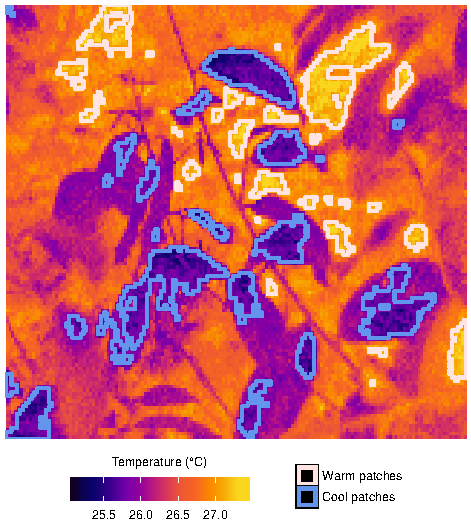
\includegraphics{./output/fig-4-2-1} 

}

\caption{Example thermal image. Pixels are shaded from cold (purple) to hot (yellow). Warm patches (outlined in pink) and cool patches (outlined in blue) were identified using the Getis-Ord local statistic of each pixel.}\label{fig:fig-4-2}
\end{figure}

\subsubsection*{Quantifying microclimates in leaf litter, tree holes and
deadwood}\label{quantifying-microclimates-in-leaf-litter-tree-holes-and-deadwood}
\addcontentsline{toc}{subsubsection}{Quantifying microclimates in leaf
litter, tree holes and deadwood}

Many ectotherms, such as amphibians, spend some or all of their time
exploiting cool microclimates inside microhabitats, which thermal images
are unable to capture. We selected three types of microhabitat known to
provide cool microclimates
\citep{scheffers_microhabitats2014, scheffers_microhabitats2014-1, gonzalez_del_pliego_thermally2016},
and placed one temperature datalogger (HOBO pendant datalogger, Onset,
model UA-001-64K or model UA-002-64K) per plot in each microhabitat
type: deadwood (\textgreater{} 10 cm stem diameter), tree holes
(\textgreater{} 2 cm at widest point of entrance hole, \textless{} 2 m
above the ground) and leaf litter (1.5 m left of the plot centre). The
hygrometer measurements of macroclimate temperature were not always
synchronised with the dataloggers inside microhabitats, hence we
additionally measured macroclimate temperature using a datalogger
suspended 1.5 m above the ground at the centre of each plot, shielded
against direct radiation and precipitation by an inverted plastic funnel
\citep{shoo_potential2010, scheffers_microhabitats2014-1}.

All dataloggers recorded temperature every 20 minutes for six
consecutive days, occurring within one week of thermal image collection.
For qualitative comparison with thermal images and to lessen the degree
of temporal autocorrelation, microclimate temperatures for each of the
three microhabitats in each plot were calculated as the median of six
daily measures, computed for each two-hour interval during the same time
period as when thermal images were collected (i.e.~04:40 to 14:40 hrs).
Our analyses focused on day-time thermal buffering, but we also ran
analogous models for the full 24 hours to explore night-time thermal
buffering (see Supplementary Text S5). In the main text, we only present
data for day-time measurements because this is most relevant to
organisms seeking to avoid extremes of heat, and because findings were
qualitatively similar. Variation in temperature for microclimates inside
microhabitats was defined as the daily range (95\textsuperscript{th}
percentile minus 5\textsuperscript{th} percentile) of raw temperatures
for each day, in each plot.

To estimate the occurrence of microclimates inside microhabitats, we
measured the volume of leaf litter, tree holes and deadwood within a 50
x 5 m subplot centred on each plot centre (60 sub-plots in total), with
the long edge running parallel to the transect. For full methodological
details see Supplementary Text S3. We divided microhabitat volume by the
total area surveyed to generate microhabitat volume per
m\textsuperscript{2} forest, for each plot.

\subsection{Variables analysed}\label{variables-analysed}

\subsubsection*{Forest structure}\label{forest-structure-1}
\addcontentsline{toc}{subsubsection}{Forest structure}

We examined the impact of selective logging on forest structure using
linear mixed effects models to compare nine structural response
variables between logged and primary forests: stand basal area of trees
and of saplings; the coefficient of variation across individual basal
areas of trees and of saplings; proportion of trees that were
dipterocarps (binomial data: dipterocarp versus non-dipterocarp);
percentage canopy cover (proportion data); and percentage vegetation
cover at ground, understorey and canopy strata (proportion data). We
found that tree stand basal area (m\textsuperscript{2}/ha) was a good
measure of changes in forest structure from logging activity (LR =
8.102, \emph{P} \textless{} 0.01; Fig. S1a; see Results for full
details), hence we use this variable as a continuous measure of
disturbance (henceforth: forest quality) in all our analyses exploring
the thermal buffering potential of logged and unlogged forests.

\subsubsection*{Macroclimate and microclimate
temperature}\label{macroclimate-and-microclimate-temperature}
\addcontentsline{toc}{subsubsection}{Macroclimate and microclimate
temperature}

Macroclimate temperature is the temperature at a relatively coarse
spatial scale, and was captured in this study using both a hygrometer
and suspended datalogger (measuring the same variable but at different
times). The macroclimate does not affect thermal buffering potential
\emph{per se}, but it does dictate the overall necessity for thermal
buffering. We modelled hygrometer and datalogger temperature separately,
including forest type (logged or primary forest) and forest quality as
explanatory variables (see Supplementary Text S4).

To assess the impact of selective logging on the ability of
microclimates to buffer organisms from macroclimate warming, we modelled
microclimate temperature against forest quality, forest type and
macroclimate temperature, including an interaction term between the
latter two variables. The slope of the relationship between microclimate
and macroclimate temperature is a measure of the rate of change. Surface
microclimate temperature refers to the 5\textsuperscript{th} percentile
of surface temperature observations (i.e.~coolest) for each plot, and
this was compared against macroclimate temperature as measured by the
hygrometer. Microclimate temperature inside leaf litter, tree holes and
deadwood refers to the two-hourly median temperature recorded by
dataloggers inside microhabitats, and this was compared against
macroclimate temperature as measured by a suspended datalogger.

To capture the impact of logging on the thermal stability of
microclimates, we modelled microclimate temperature range against forest
type and forest quality. For surface microclimates, the range was the
daily range of surface temperature observations (the
5\textsuperscript{th} percentiles, i.e.~coolest surface temperatures).
For microclimates inside microhabitats, the range was the daily range
(95\textsuperscript{th} percentile minus 5\textsuperscript{th}
percentile) of the raw temperature observations. All models were run
separately for surface, leaf litter, tree hole and deadwood
microclimates.

\subsubsection*{Microclimate
availability}\label{microclimate-availability}
\addcontentsline{toc}{subsubsection}{Microclimate availability}

Microclimate occurrence was modelled separately for surface
microclimates (i.e.~the average surface area of cool patches), and those
inside leaf litter, tree holes and deadwood (each quantified by their
average volume per m\textsuperscript{2} forest). The thermal diversity
of surface microclimates was captured by the temperature range between
the warmest warm patch and the coolest cool patch. The spatial
configuration of surface microclimates refers to the Aggregation Index
of cool patches (binomial data: edges shared by cool patches versus
edges not shared by cool patches). For all models, the fixed effects
were forest type (logged or primary forest) and forest quality
(i.e.~tree stand basal area).

\subsection{Statistical analyses}\label{statistical-analyses}

All data were analysed using mixed effects models in R \citep[version
3.3.0;][]{r_core_team_r:2017}. To account for spatial pseudoreplication,
forest structure models included `site' as a random intercept term, and
all other models included `plot' nested within `site'. Temperature data
were recorded at multiple time points, hence the full models were
visually assessed for evidence of temporal autocorrelation of residuals
\citep[function `acf' in the nlme package;][]{pinheiro_nlme:2017}, and a
correlation structure for both date and time was incorporated where
necessary \citep[the specific structure was chosen using
AIC;][]{zuur_mixed2009}. For binomial data (proportion of dipterocarps
and surface microclimate Aggregation Index) we used generalized linear
mixed effects models (GLMMs) with a binomial error distribution, fitted
using the package lme4 \citep{bates_fitting2015} and tested for
overdispersion. Diagnostic plots were assessed for all models to confirm
model fit and, where necessary, we modified the variance structure of
the residuals \citep{zuur_mixed2009} and transformed variables to
normality. For true proportion data (percentage canopy cover and
percentage vegetation cover), the transformation used was a modification
of the empirical logit \citep{warton_arcsine2011}.

For all models, statistical significance was inspected using likelihood
ratio tests, dropping each fixed effect in turn and comparing it to the
full model \citep{zuur_mixed2009}. The significance of main effects
involved in an interaction was assessed in the same way, except reduced
models were compared to a full model without the interaction term. The
basic structure for most response variables (RV) was:

\texttt{RV\ \textasciitilde{}\ forest\_type\ +\ forest\_quality\ +\ (1\textbar{}transect/plot)\ +\ cor(\textasciitilde{}\ date\_time\textbar{}transect/plot)}

\section{Results}\label{results-1}

\subsection{Changes in forest structure after
logging}\label{changes-in-forest-structure-after-logging}

Following two rounds of commercial selective logging, tree stand basal
area -- our measure of forest quality -- was 23.4
m\textsuperscript{2}/ha in logged forest, compared to 39.5
m\textsuperscript{2}/ha in primary forest (LR = 8.102, \emph{P}
\textless{} 0.01; Fig. S1a). Logged forests thus contained far fewer
large trees than did primary forests. There were also more large
saplings in logged forest (9.55 m\textsuperscript{2}/ha) than in primary
forests (6.77 m\textsuperscript{2}/ha; LR = 4.239, \emph{P} \textless{}
0.05; Fig. S1b), and trees were less variable in size (LR = 13.038,
\emph{P} \textless{} 0.001; Fig. S1c). There was no difference between
forest types in terms of the variability of size among saplings (LR =
0.114, \emph{P} = 0.736; Fig. S1d).

Changes to forest structure from selective logging were also evident in
the overall amount of vegetation cover. Although there was no observed
difference between logged forest and primary forest in percentage
vegetation at ground level (LR = 2.758, \emph{P} = 0.097; Fig. S1g), the
proportion of trees that were dipterocarps (Χ² = 2.42, \emph{P} = 0.12;
Fig. S1e) or the percentage canopy cover (LR = 0.874, \emph{P} = 0.35;
Fig. S1f), we did find that percentage vegetation cover was higher in
primary forest than in logged forest in both the understorey (primary =
68.2\%; logged = 54.4\%; LR = 5.288, \emph{P} \textless{} 0.05; Fig.
S1h), and in the canopy (primary = 23.1\%; logged = 8.6\%; LR = 9.174,
\emph{P} \textless{} 0.01; Fig. S1i). Thus, 9-12 years after logging
there were significant differences in forest structure between logged
and primary forests. This was especially true for the components of
forest structure that typically indicate the presence of large, mature
trees and high structural complexity, and which might be expected to
influence microclimates and the availability of microhabitats.

\subsection{Macroclimate and microclimate temperature in logged and
primary
forest}\label{macroclimate-and-microclimate-temperature-in-logged-and-primary-forest}

Despite differences in forest structure, we found no difference in
macroclimate temperature of logged and primary forests, whether measured
by the hygrometer (LR = 0.081, \emph{P} = 0.776; Fig. S2a) or suspended
datalogger (LR = 0, \emph{P} = 0.983; Fig. S2b). Macroclimate
temperature was also consistent across varying levels of forest quality,
for temperature measured via the hygrometer (LR = 0.022, \emph{P} =
0.883; Fig. S2a) and suspended datalogger (LR = 0.527, \emph{P} = 0.468;
Fig. S2b). Thus, the necessity for thermal buffering was comparable
between the two forest types.

Absolute microclimate temperature was comparable between forest types
for all of the microclimates considered: surface (LR = 0.447, \emph{P} =
0.504; \autoref{fig:fig-4-3}), deadwood (LR = 0.206, \emph{P} = 0.65;
Fig. 3f), tree holes (LR = 2.759, \emph{P} = 0.097; Fig. 3g) and leaf
litter (LR = 1.616, \emph{P} = 0.204; Fig. 3h). We found that the
relationship between microclimate temperature and macroclimate
temperature was slightly steeper in primary forest compared to logged
forest for deadwood (LR = 7.268, \emph{P} \textless{} 0.01; Fig. 3b),
tree holes (LR = 13.657, \emph{P} \textless{} 0.001; Fig. 3c) and leaf
litter (LR = 28.914, \emph{P} \textless{} 0.001; Fig. 3d). However, for
1°C macroclimate warming (from the median value) the maximum difference
in microclimate warming between forest types was \textless{} 0.1°C, and
no such interaction was apparent for surface microclimates (LR = 1.197,
\emph{P} = 0.274; Fig. 3a). Similarly, for a 1 m\textsuperscript{2}/ha
increase in forest quality (i.e.~tree stand basal area), tree hole
temperature was slightly warmer (LR = 4.661, \emph{P} \textless{} 0.05;
Fig. 3g), but the size of this effect was negligible (+0.00194°C), and
not evident for other microclimates (\emph{P} \textgreater{} 0.05; Fig.
3e-h). Thus we conclude that effects of logging on microclimate
temperature were generally not evident, or minimal.

The final facet of microclimate temperature that we considered was daily
temperature variation. This too was comparable between logged and
primary forests for microclimates at the surface (LR = 0.437, \emph{P} =
0.508; Fig. 4a), as well as those inside deadwood (LR = 0.02, \emph{P} =
0.889; Fig. 4b), tree holes (LR = 3.242, \emph{P} = 0.072; Fig. 4c) and
leaf litter (LR = 2.449, \emph{P} = 0.118; Fig. 4d). Microclimate
temperature variation was also consistent across different levels of
forest quality (\emph{P} \textgreater{} 0.05; Fig. 4).

In summary, selective logging had little observed impact on absolute
microclimate temperature or its daily variation. There was some evidence
that thermal buffering potential was slightly enhanced for deadwood,
tree holes and leaf litter inside logged forest, but the effects were
extremely small and not evident for microclimates at the surface.

\begin{center}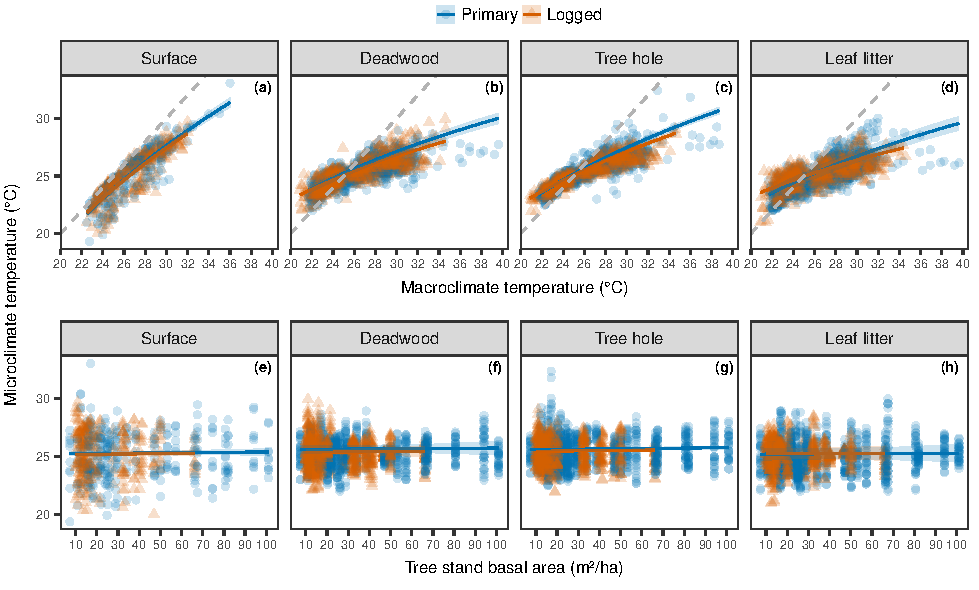
\includegraphics{./output/fig-4-3-1} \end{center}

``Comparison between primary forest (blue) and logged forest (orange) in
terms of: (a-d) the relationship between microclimate temperature and
macroclimate temperature; and (e-h) absolute microclimate temperature
across varying levels of forest quality (measured as tree stand basal
area). Microclimates were measured at the surface (a, e), and inside
deadwood (b, f), tree holes (c, g) and leaf litter (d, h). The grey
dashed lines in panels a-d indicate zero temperature buffering, where
the microclimate temperature is equal to the macroclimate temperature.
In all panels, shaded bands are 95\% confidence intervals.''

\begin{center}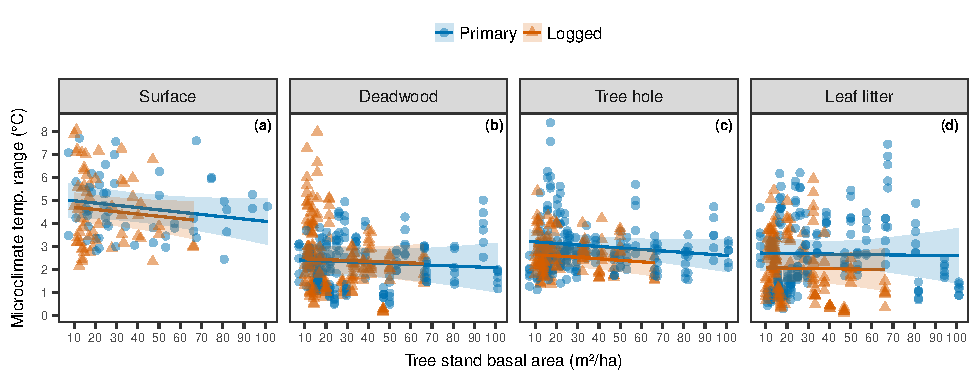
\includegraphics{./output/fig-4-4-1} \end{center}

``The influence of forest type (primary or logged) and forest quality
(measured as tree stand basal area) on microclimate temperature range.
Daily range for surface microclimates (a) was calculated as the
difference between the maximum and the minimum microclimate temperature
(itself calculated as the 5\textsuperscript{th} percentile temperature
across four photos taken at each visit to each plot). For microclimates
inside deadwood (b), tree holes (c) and leaf litter (d), the daily range
was the difference between the 95\textsuperscript{th} percentile and
5\textsuperscript{th} percentile of raw temperature measurements.
Primary forest data points are depicted as blue circles and logged
forest as orange triangles. Shaded bands represent 95\% confidence
intervals.''

\subsection{Microclimate availability in logged and primary
forest}\label{microclimate-availability-in-logged-and-primary-forest}

The thermal buffering potential within a habitat depends not only on the
temperature of microclimates relative to the macroclimate, but also on
the overall availability and thermal diversity of those microclimates.
The occurrence of surface microclimates was not impacted by forest type
(LR = 0.872, \emph{P} = 0.35; Fig. 5b), and the average volume of
microhabitats (per m\textsuperscript{2} forest) was similar in logged
and primary forest for deadwood (LR = 0.263, \emph{P} = 0.608; Fig. 5d),
tree holes (LR = 3.053, \emph{P} = 0.081; Fig. 5e) and leaf litter (LR =
0.162, \emph{P} = 0.687; Fig. 5f). There was no observed impact of
forest quality on the occurrence of surface microclimates (LR = 1.324,
\emph{P} = 0.25; Fig. 5b) or the volume of deadwood (LR = 3.78, \emph{P}
= 0.052; Fig. 5d) and tree holes (LR = 2.172, \emph{P} = 0.141; Fig.
5e). In contrast, we found that leaf litter volume increased by 12.3
cm\textsuperscript{3}/m\textsuperscript{2} for a 1
m\textsuperscript{2}/ha increase in forest quality (i.e.~tree stand
basal area; LR = 7.056, \emph{P} \textless{} 0.01; Fig. 5f).

Using thermal images we were able to quantify the thermal diversity and
spatial configuration of surface microclimates. Thermal diversity has a
bearing on the diversity of organisms that are able to find
microclimates meeting their thermal requirements (which vary according
to species, age, time of day, seasonality, etc.). Spatial configuration
influences the ease with which organisms can utilise microclimates. We
found that the temperature range spanned by surface microclimates (both
warm and cool patches) was comparable between logged and primary forests
(LR = 0.276, \emph{P} = 0.599; Fig. 5a) and with varying forest quality
(LR = 3.552, \emph{P} = 0.059; Fig. 5a). The same was true for the
Aggregation Index of cool surface patches, both between logged and
primary forest (Χ² = 0.312, \emph{P} = 0.576; Fig. 5c) and with
different levels of forest quality (Χ² = 0.183, \emph{P} = 0.669; Fig.
5c).

Overall, the availability of microclimates was minimally affected by
selective logging, regardless of whether microclimates were located at
the surface or inside microhabitats. This was true for various different
components of microclimate availability, including their occurrence,
thermal diversity and spatial configuration.

\begin{center}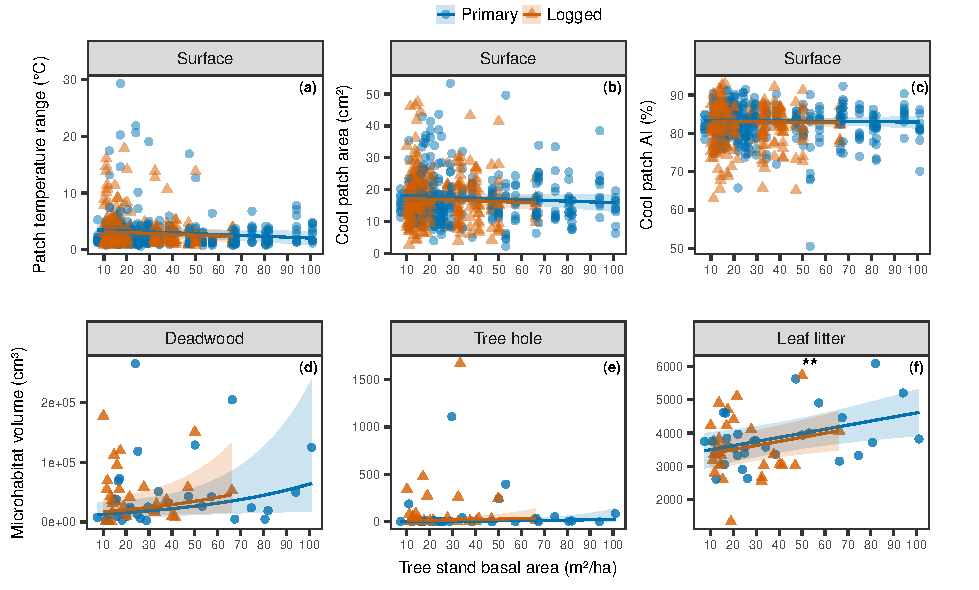
\includegraphics{./output/fig-4-5-1} \end{center}

The influence of forest type (primary or logged forest) and forest
quality (measured as tree stand basal area) on microclimate
availability. Results for surface microclimates (top row) include: the
temperature range from the warmest warm patch to the coolest cool patch
(a); the average surface area of cool patches (b); and the Aggregation
Index of cool patches (c). The volume (per m\textsuperscript{2} forest)
of microhabitats typically associated with microclimates (bottom row) is
shown for deadwood (d), tree holes (e) and leaf litter (f). Primary
forest data points are depicted as blue circles and logged forest as
orange triangles. Shaded bands represent 95\% confidence intervals.
Asterisks in panel f denote a statistically significant difference at
0.001 \textless{} \emph{P} \textless{} 0.01 (**).

\section{Discussion}\label{discussion-1}

Forest degradation by commercial selective logging affects huge expanses
of the tropics \citep{asner_contemporary2009, lewis_increasing2015}.
Southeast Asia has experienced the most intensive selective logging of
all tropical rainforests \citep{lewis_increasing2015}, and in our study
area \textasciitilde{}145 m\textsuperscript{3} of timber was removed per
hectare. Despite these forests having only a maximum of 12 years
post-logging recovery \citep{fisher_cost-effective2011}, and the
coincidental occurrence during data collection of abnormally hot and dry
conditions associated with the strongest El Niño-Southern Oscillation
(ENSO) event since 1998 \citep{noaa2015}, we found very few thermal
differences associated with selective logging. This is an important
finding for tropical conservation because it suggests that the potential
for thermal buffering will not limit the ability of selectively logged
forests to maintain high biodiversity under climate change.

\subsection{Forest structure}\label{forest-structure-2}

At a local scale (m to ha), climate is highly dependent upon vegetation
\citep{oke_boundary1987, sears_world2011}. Selective logging operations
generally target larger and older trees, leading to many associated
changes in vegetation structure
\citep{okuda_effect2003, kumar_effects2005, edwards_maintaining2014}. A
clear signal of historical logging in our study area was a reduction in
stand basal area of mature trees by 40.8\% \citep[Fig.
S1a;][]{berry_impacts2008}, accompanied by reduced variation in tree
basal area (Fig. S1c), and reduced vegetation cover at ≥ 15 m height
(Fig. S1h,i). The increase in stand basal area of saplings by 41.1\%
(Fig. S1b) is evidence that there has been substantial natural
regeneration in the intervening years.

\subsection{Macroclimate and microclimate
temperature}\label{macroclimate-and-microclimate-temperature-1}

Although primary forest contained more large trees (Fig. S1a), the
absence of any long-term effect of selective logging on percentage
canopy cover (Fig. S1f) suggests that forest vegetation as a whole --
regardless of how it was distributed vertically -- intercepted
comparable amounts of incoming solar radiation in both logged and
primary forests. This finding is in keeping with previous studies
observing rapid horizontal canopy growth following selective logging
\citep[e.g.][]{asner_canopy2004}. Alternatively, vegetation in logged
forest may have intercepted less incoming radiation than in primary
forest (i.e.~if there was less vegetation overall), but reflected a
greater proportion of what was intercepted, owing to the higher albedo
of habitats with an abundance of non-tree species
\citep{oke_boundary1987, davin_climatic2010, edwards_maintaining2014}.
In either case (or in combination), given comparable levels of solar
radiation reaching the forest floor of logged and primary forests, it
follows that the temperature at coarse and fine scales (macroclimate and
microclimate temperatures) should also be comparable (Fig. 3 and Fig.
S2).

The temperature of cool microclimates relative to average conditions is
what largely determines their ability to buffer macroclimate warming
\citep{scheffers_microhabitats2014-1, gonzalez_del_pliego_thermally2016, shi_framework2016}.
Given that selective logging did not affect absolute temperature of the
macroclimate (Fig. S2) or microclimates (Fig. 3), we can infer that
there was no overall effect of selective logging on the difference
between micro- and macroclimate temperature. There was also no evidence
that selective logging impacted overall daily variation in microclimate
temperature (Fig. 4). There were some impacts of logging on the
relationship between microclimate and macroclimate temperature for
microclimates inside deadwood, tree holes and leaf litter (Fig. 3), but
the effect sizes for these interactions were extremely small. The
maximum difference in microclimate warming between logged and primary
forests was \textless{} 0.1°C for 1°C of macroclimate warming. As such,
we conclude that even when selective logging had a statistically
significant influence on thermal buffering potential, the effect was
small and of limited biological relevance.

\subsection{Microclimate
availability}\label{microclimate-availability-1}

Even if microclimates are present and effective at buffering temperature
change, overall rarity or isolation could render them functionally
redundant to some species
\citep{sears_world2011, sears_configuration2016}. We demonstrate that
lower forest quality was associated with less leaf litter \citep[Fig. 5;
cf.][]{saner_reduced2009}, but forest quality and forest type had little
effect on the occurrence of microclimates at the surface or inside
deadwood and tree holes. This is contrary to expectations from previous
studies \citep{ball_tree1999, blakely_tree2008}. However, high volumes
of deadwood could be maintained in logged forest by lower decomposition
rates
\citetext{\citealp{ewers_logging2015}; \citealp{yeong_leaf2016}; \citealp[but
see][]{herault_modeling2010}}, and large remnant pieces from harvest
operations. In undisturbed forests, tree holes tend to be associated
with larger, older trees
\citep{lindenmayer_cavity2000, blakely_tree2008}. A comparable quantity
of tree holes might be found in logged forests because of damage from
logging operations \citep{edwards_maintaining2014}, increased wind in
gaps \citep{chen_growing-season1995} and remnant large trees that were
specifically avoided by logging companies because of hollow boles.
Additionally, we assessed tree holes in the understorey only, and
differences may well manifest at higher forest strata.

The availability of microclimates to organisms is also influenced by
their thermal diversity and distribution in space. We found that patches
of warm and cool microclimates on the surface of the forest floor
spanned a temperature range of about 3°C, regardless of logging activity
(Fig. 5a). Cool patches were generally highly clustered in space
(Aggregation Index of 83.3\%), but this was not affected by logging
(Fig. 5c). Thermal diversity and spatial configuration of microclimates
are relatively novel facets of thermal buffering potential \citep[but
see:][]{caillon_warming2014, sears_configuration2016, faye_toolbox2016};
they are likely determined by the composition of the forest floor and
the relative radiative properties of these different components
\citep[e.g.~bare soil versus leaves versus
water;][]{oke_boundary1987, snyder_analyzing2004}. We therefore suggest
that these characteristics of the forest floor were comparable between
forests despite the large differences in forest structure that were
evident after logging.

\subsection{Caveats and future research
directions}\label{caveats-and-future-research-directions}

The potential for thermal buffering and its general necessity are
influenced by moisture levels, as well as temperature
\citep{mclaughlin_hydrologic2017}. Many ectotherms, including amphibians
\citep{duellman_biology1986} and isopods \citep{hassall_predicting2010},
can survive in hot temperatures for longer if relative humidity is
sufficiently high to prevent desiccation. Although we did not measure
fine-scale vapour pressure deficit (a variable combining both
temperature and relative humidity), we did find that coarse-scale vapour
pressure deficit measurements from the hygrometer and from hygrochron
iButtons (Supplementary Text S4) showed little variation within or
between forests (Fig. S2).

Relative climates in primary and logged forests could be very different
above the understorey, which we were unable to capture in our study.
Some ectotherms move down from the upper strata to exploit more
favourable temperatures lower down \citep{scheffers_increasing2013}.
Hence, if temperatures in higher strata are in fact hotter in logged
forest compared to primary forest, it is possible that species could
move to utilise the favourable temperatures of the understorey of logged
forest that we demonstrate here, potentially resulting in a `flattening'
of species' vertical distributions.

While thermal cameras are an important addition to the toolbox of
microclimate research \citep{faye_toolbox2016}, it is also important to
remember that they are just one element. Thermal cameras are well-suited
to capturing temperature at a very fine-scale and with inherent spatial
information, but differences in 3D topography of a surface could affect
results (e.g.~the real distance between neighbouring pixels can be more
than is apparent in the 2D image). Additionally, although thermal
cameras are ideal for measuring surface temperatures, they have a
limited capacity to capture sub-surface temperatures, and hence we have
used thermal imagery in combination with dataloggers.

The ability of selectively logged tropical forests to retain current
levels of biodiversity will critically depend on their ability to
protect species from the impacts of increasingly severe climate change.
As average temperatures increase over this century, so too will the
intensity and frequency of extreme climatic events. Thermal buffering
will likely be crucial in allowing species to move locally to avoid
suboptimal climates. We sampled in some of the most intensively logged
forest in the tropics, during abnormally hot and dry conditions of a
severe ENSO event; it is highly unlikely that our study would have
failed to detect any appreciable thermal differences between primary and
logged forests had they existed. Regardless of whether commercially
selectively logged forests remain biologically or structurally
distinctive from undisturbed forests, this study shows for the first
time that they are functionally equivalent in the provisioning of cool
microclimates, and underscores their vital role in conservation both now
and under future climate warming.

\section{Acknowledgements}\label{acknowledgements-1}

Thanks to staff at Danum Valley Field Centre for logistical support; and
Azlin Bin Sailim, Jessica Olid and Chloe Walker-Trivett for field
assistance. R.A.S. was funded by a NERC studentship through the ACCE
(Adapting to the Challenges of a Changing Environment) Doctoral Training
Partnership (Grant No. NE/L002450/1).

\section{Data availability}\label{data-availability}

Data available from the University of Sheffield Online Research Data
repository (DOI: 10.15131/shef.data.5414629).

\chapter{The impact of recent forest cover change on climate
connectivity in the
tropics}\label{the-impact-of-recent-forest-cover-change-on-climate-connectivity-in-the-tropics}

\begin{figure}[!htb]
\centering
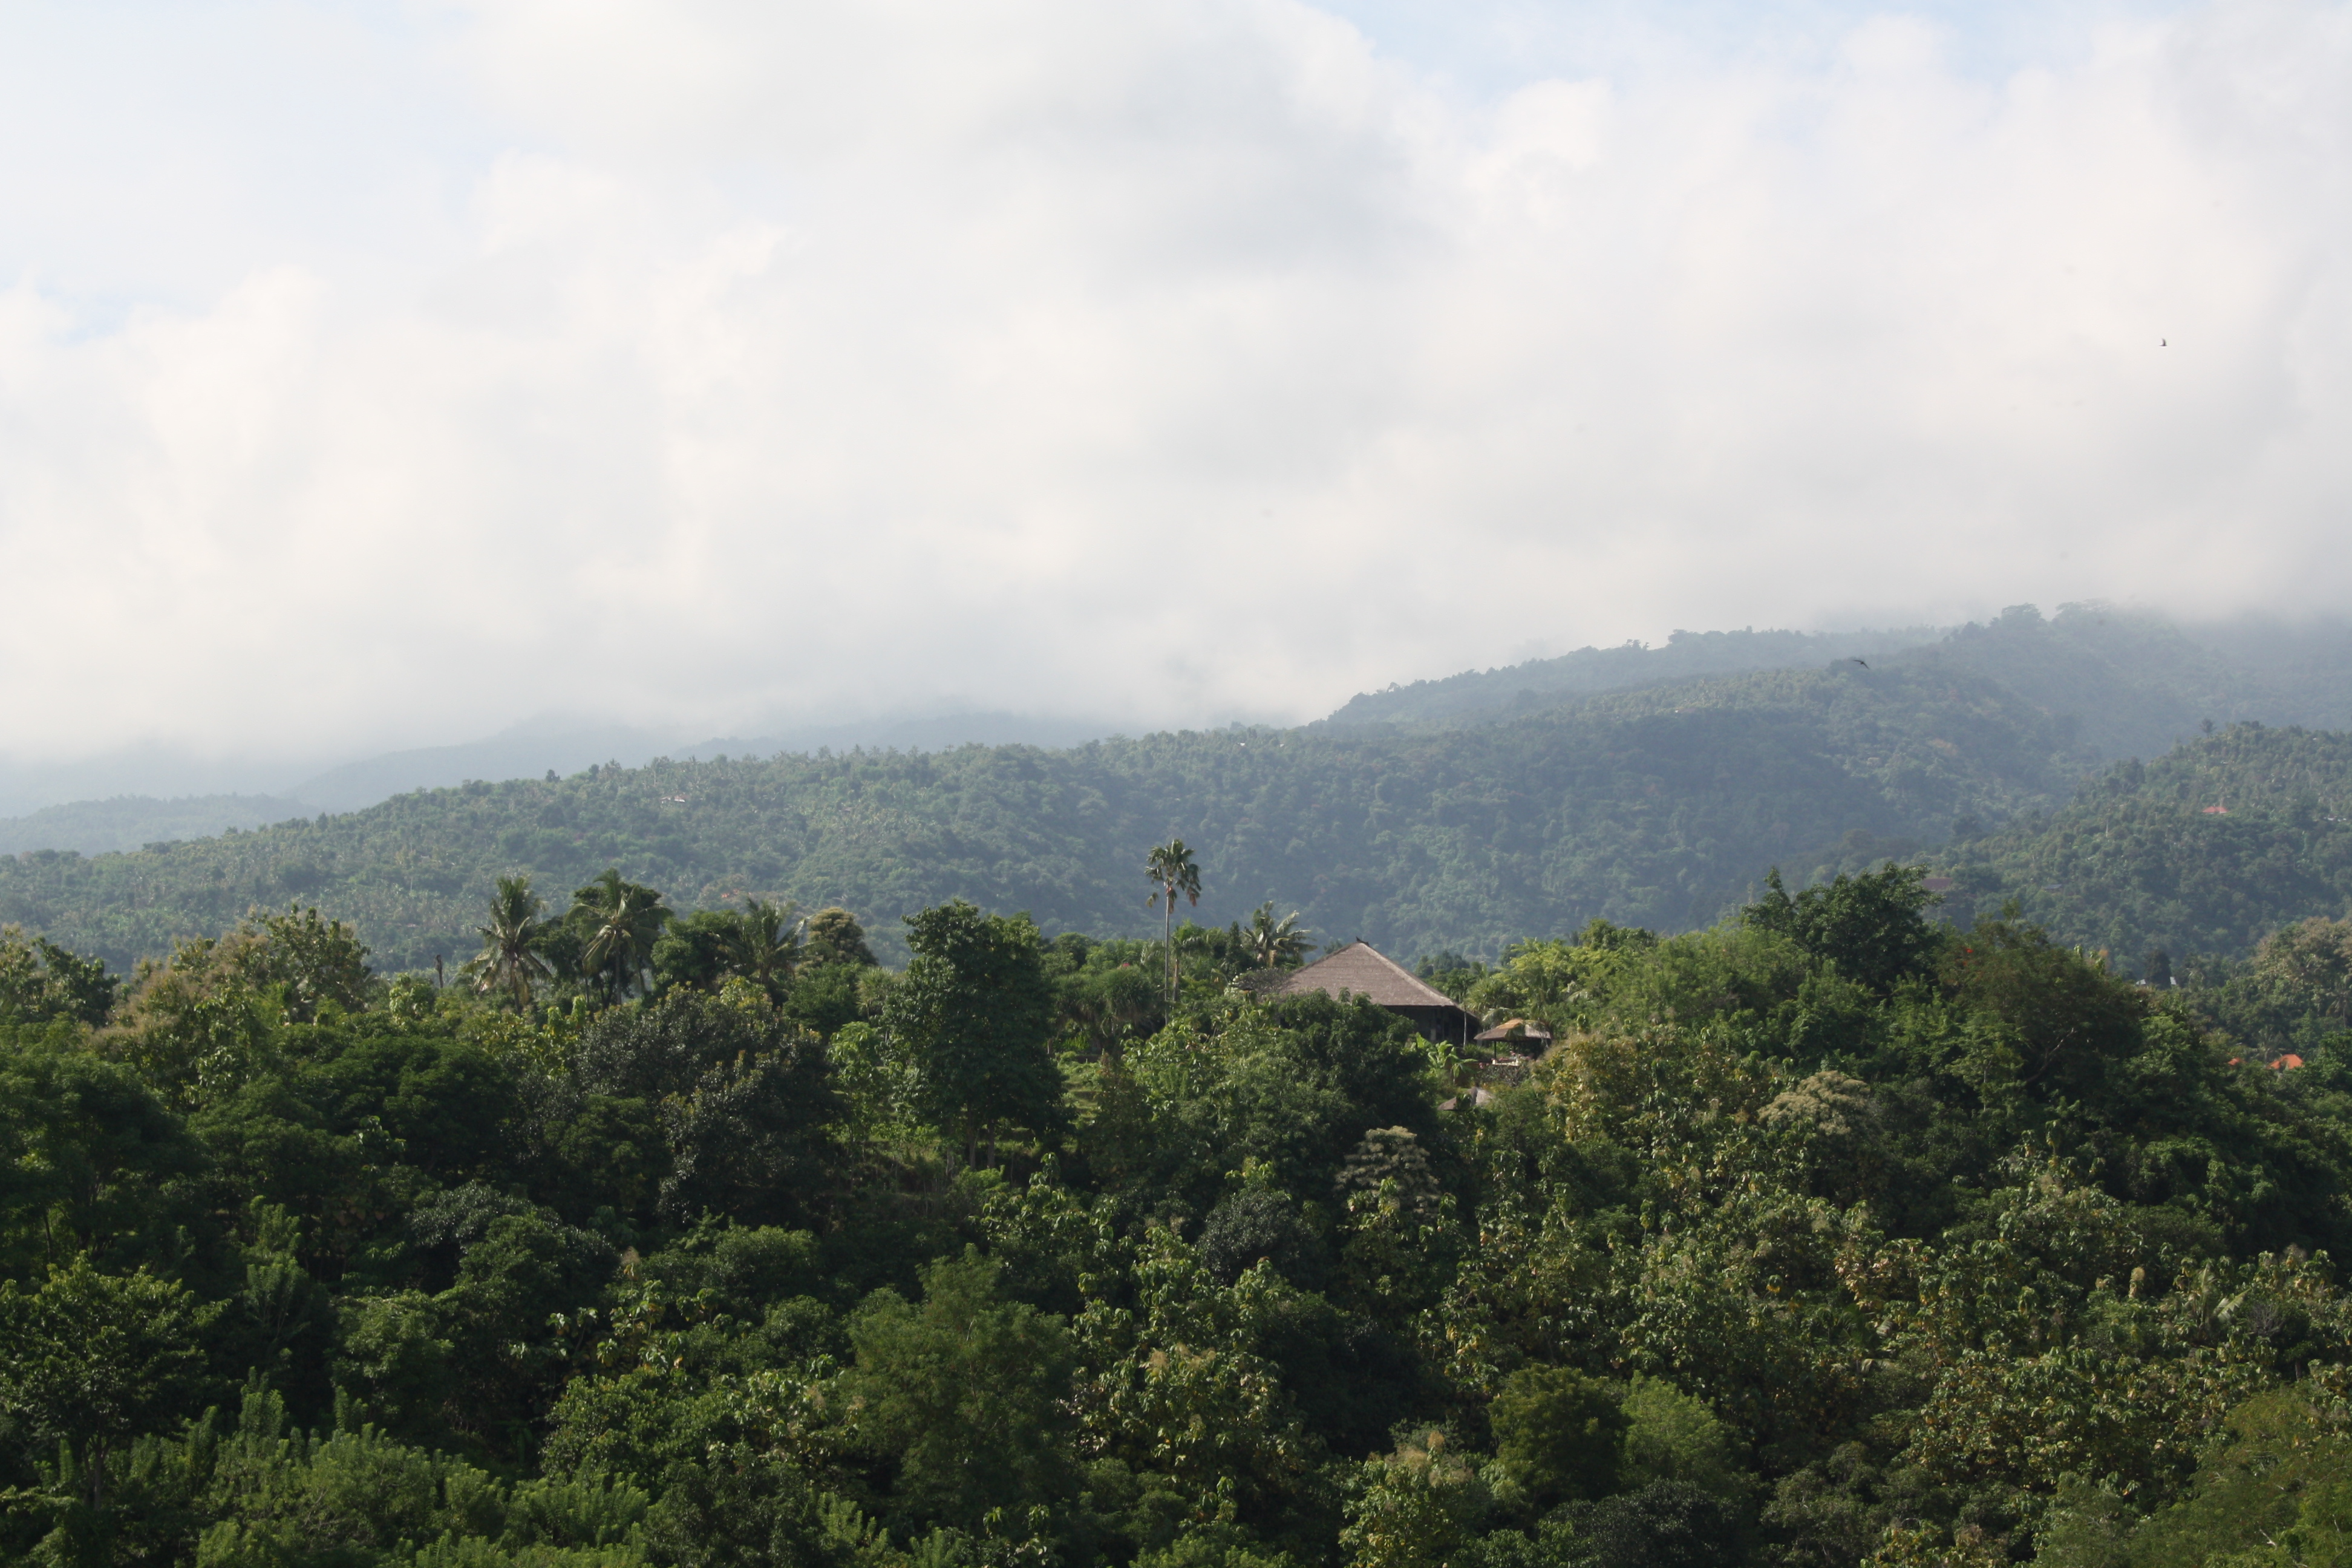
\includegraphics[width=15cm]{pics/landscape1.jpg}
\caption*{Mixed use tropical landscape in Bali.}
\end{figure}

\pagebreak

\chapter{Discussion}\label{discussion-2}

\begin{figure}[!htb]
\centering
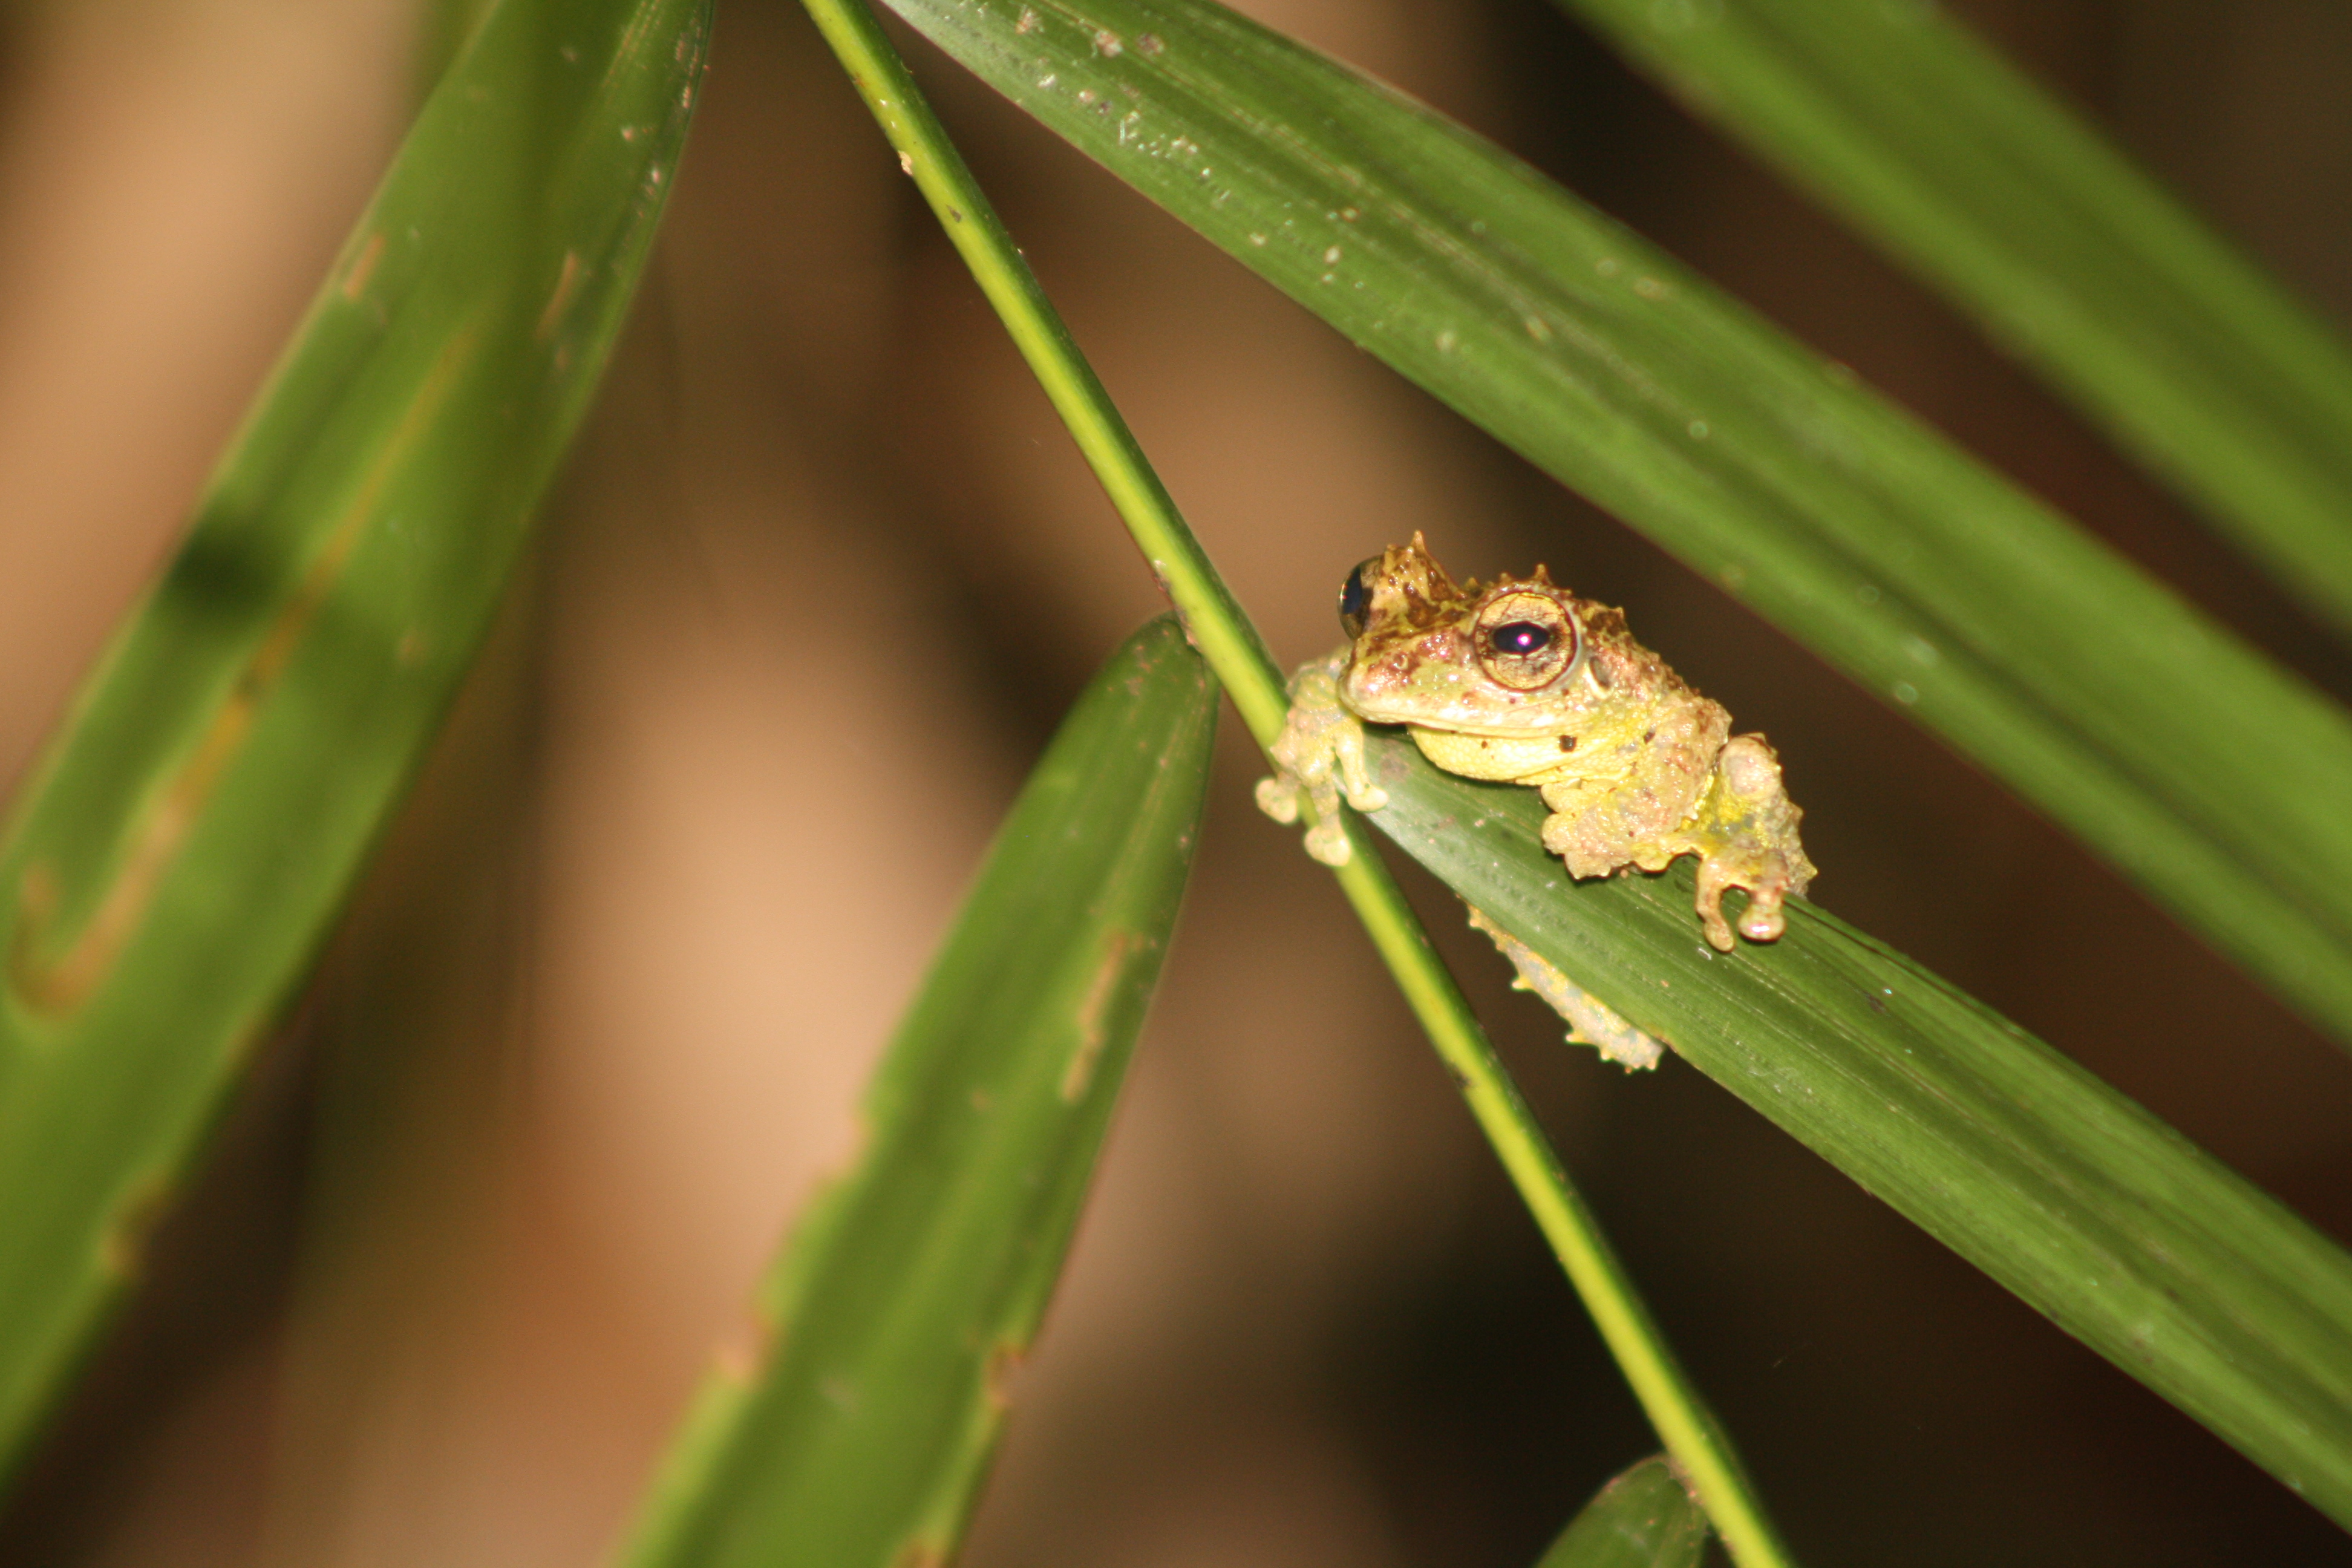
\includegraphics[width=13cm]{pics/Frilled_tree_frog.jpg}
\caption*{Frilled tree frog (\textit{Kurixalus appendiculatus}).}
\end{figure}

\pagebreak

\clearpage
\appendix
\fancyhead[R]{Appendix \thechapter} \addappheadtotoc
\setcounter{figure}{0} \makeatletter 
\renewcommand{\thefigure}{A1.\@arabic\c@figure} \makeatother

\chapter{Supporting information for Chapter
2}\label{supporting-information-for-chapter-2}

\section{Impact of unbalanced sampling}\label{text-A-1-1}

\subsection{Methods}\label{methods-1}

Some studies contributed substantially more temperature observations
than others. To test whether these studies were unduly influencing our
results, we established a threshold over which a given land-use type, in
a given study, was deemed to have a disproportionate number of
associated temperature observations. The threshold used --- 2,071
observations --- was the mean number of observations across all unique
combinations of land-use type and study identity (55 in total). The same
number of observations (2,071) was then randomly re-sampled from each of
the land-use type and study combinations that exceeded the threshold.
With this reduced and more balanced dataset we repeated the main
analysis (see `Statistical analysis' in main text for more details),
modelling local day-time temperature (`temp\_day') against land-use type
(`LUT'), position relative to ground-level (`position') and season. The
final model structure was unchanged, and included a random slope for
land-use type and random intercept with respect to the identity of the
study (`studyID') from which data originated:

\texttt{lmer(temp\_day\ \ \textasciitilde{}\ LUT*position\ +\ LUT*season\ +\ (LUT\textbar{}studyID))}

\subsection{Results}\label{results-2}

All results were qualitatively unchanged from those derived using the
full dataset. Local day-time temperature was warmer in altered land-use
types, compared to primary forest (LMM, Χ\textsuperscript{2} = 32.19, df
= 4, P \textless{} 0.001; \autoref{fig:fig-A-1-3}). Averaged across
above- and below-ground, and across seasons, the temperature
differential was greatest in cropland (7.7°C), followed by pasture
(6.4°C), plantation (3.2°C) and degraded forest (0.9°C). The
relationship between land-use type and temperature interacted with both
position relative to ground level (LMM, Χ\textsuperscript{2} = 681, df =
4, P \textless{} 0.001; \autoref{fig:fig-A-1-3}A) and season (LMM,
Χ\textsuperscript{2} = 105.63, df = 4, P \textless{} 0.001;
\autoref{fig:fig-A-1-3}B). Specifically, the difference between altered
land-use types and primary forest was greater above-ground than
below-ground (\autoref{fig:fig-A-1-3}A), and variable between seasons
according to the land-use type (\autoref{fig:fig-A-1-3}B).

\pagebreak

\section{Supplementary figures}\label{supplementary-figures}

\begin{figure}
\centering
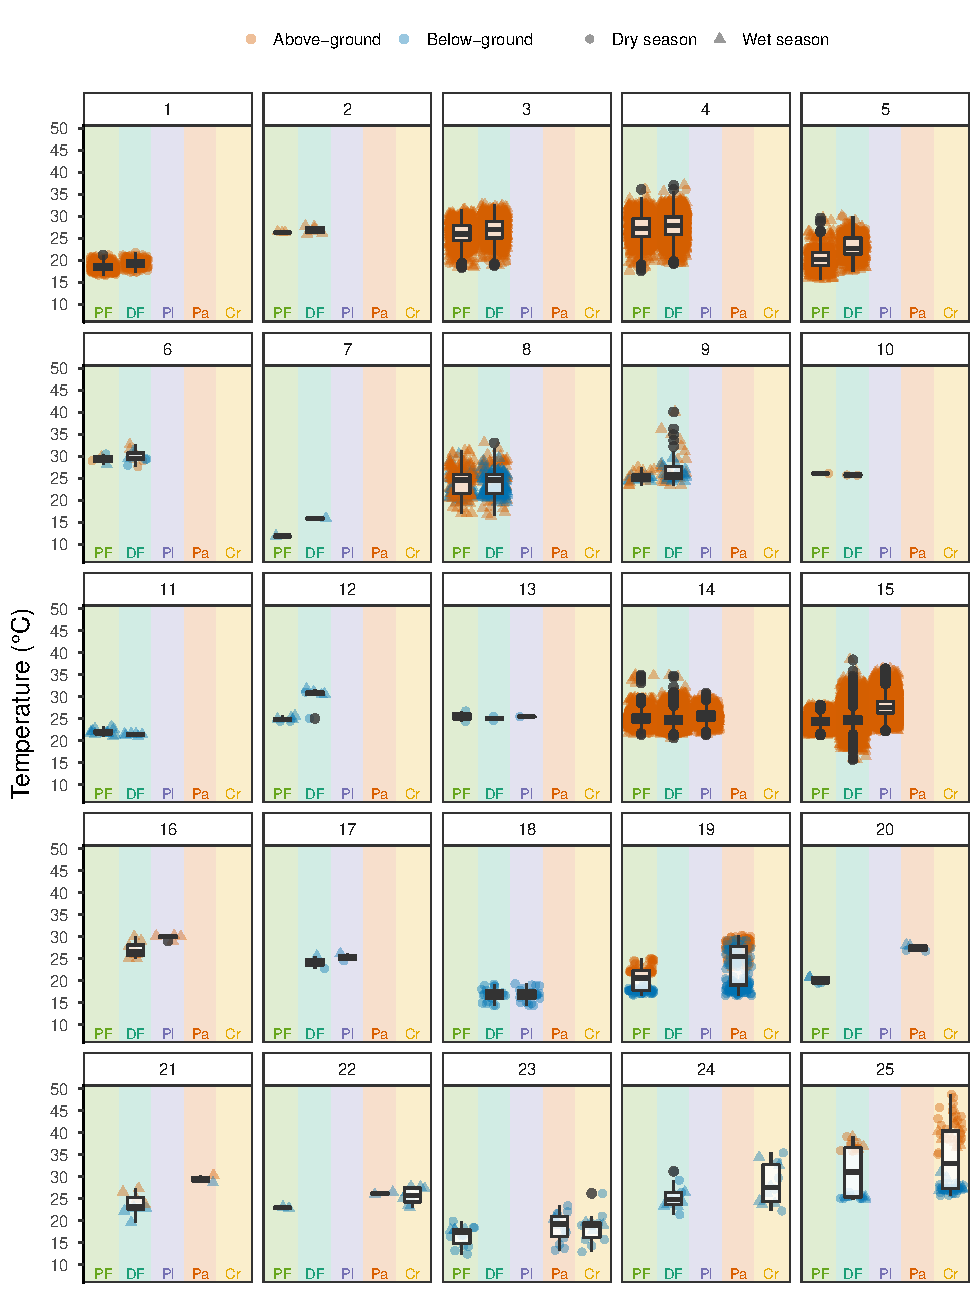
\includegraphics{./output/fig-A-1-1-1.pdf}
\caption{\label{fig:fig-A-1-1}Day-time temperature against land-use type for
each study contributing data to the analyses. Panel numbers refer to the
study number in the reference list below. Land-use types are: primary
forest (PF), degraded forest (DF), plantation (Pl), pasture (Pa) and
cropland (Cr). Panels are ordered by the combination of land-use types
for which data was available: (1-12) PF + DF; (13-15) PF + DF + Pl;
(16-18) DF + Pl; (19-20) PF + Pa; (21) DF + Pa; (22-23) PF + Pa + Cr;
and (24-25) DF + Cr. Shading of points indicates temperatures measured
above-ground (orange) or below-ground (blue), and point symbol indicates
temperatures measured during the dry season (circles) or wet season
(triangles).}
\end{figure}

\begin{figure}
\centering
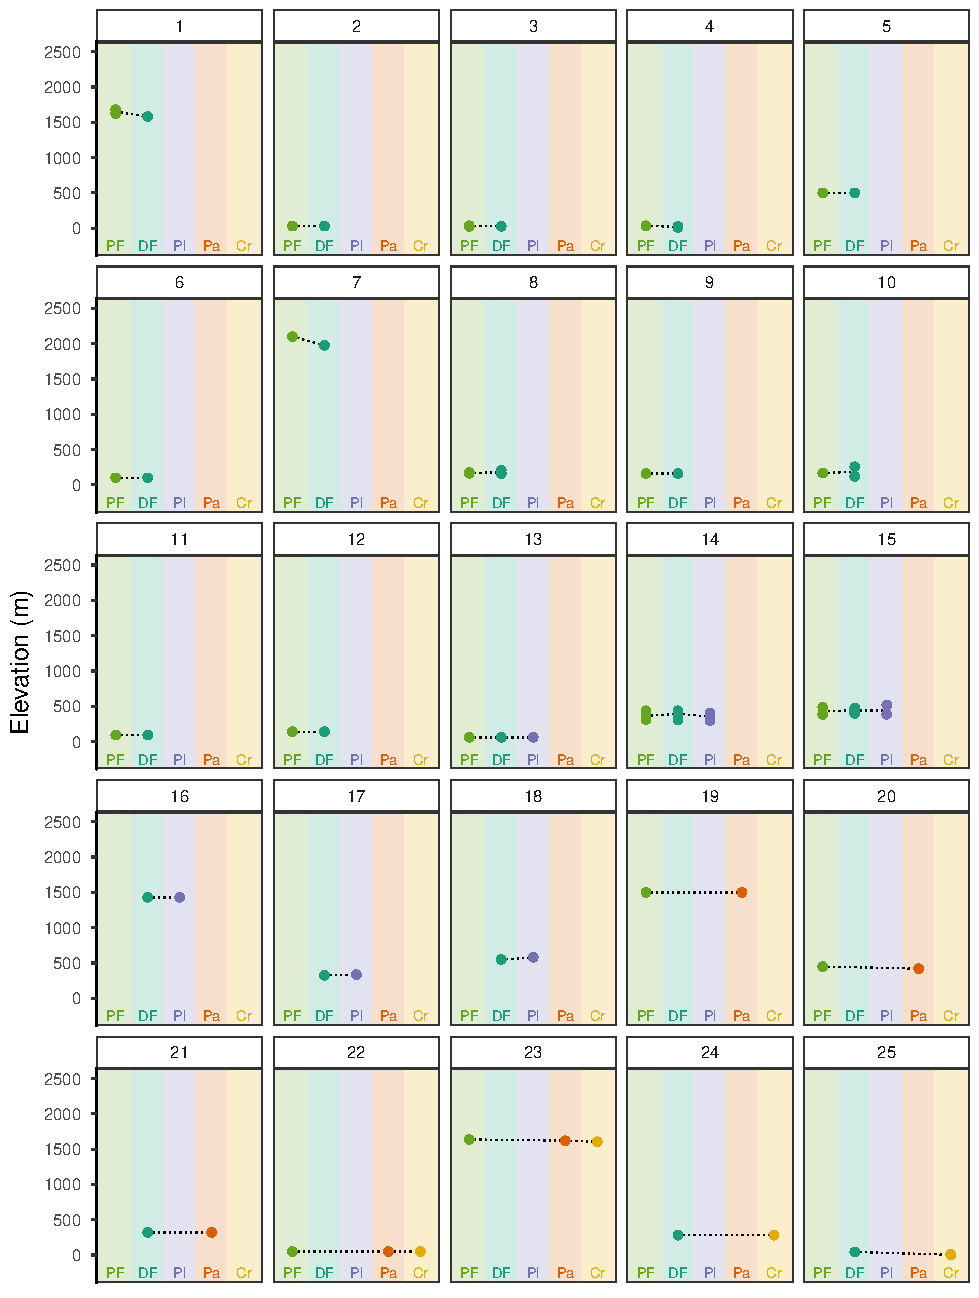
\includegraphics{./output/fig-A-1-2-1.pdf}
\caption{\label{fig:fig-A-1-2}Site elevation against land-use type for each
study contributing data to the analyses. Panel numbers refer to the
study number in the reference list below. Land-use types are: primary
forest (PF), degraded forest (DF), plantation (Pl), pasture (Pa) and
cropland (Cr). Panels are ordered by the combination of land-use types
for which data was available: (1-12) PF + DF; (13-15) PF + DF + Pl;
(16-18) DF + Pl; (19-20) PF + Pa; (21) DF + Pa; (22-23) PF + Pa + Cr;
and (24-25) DF + Cr. Dotted black lines connect the mean elevation of
all the sites within each land-use type.}
\end{figure}

\begin{figure}
\centering
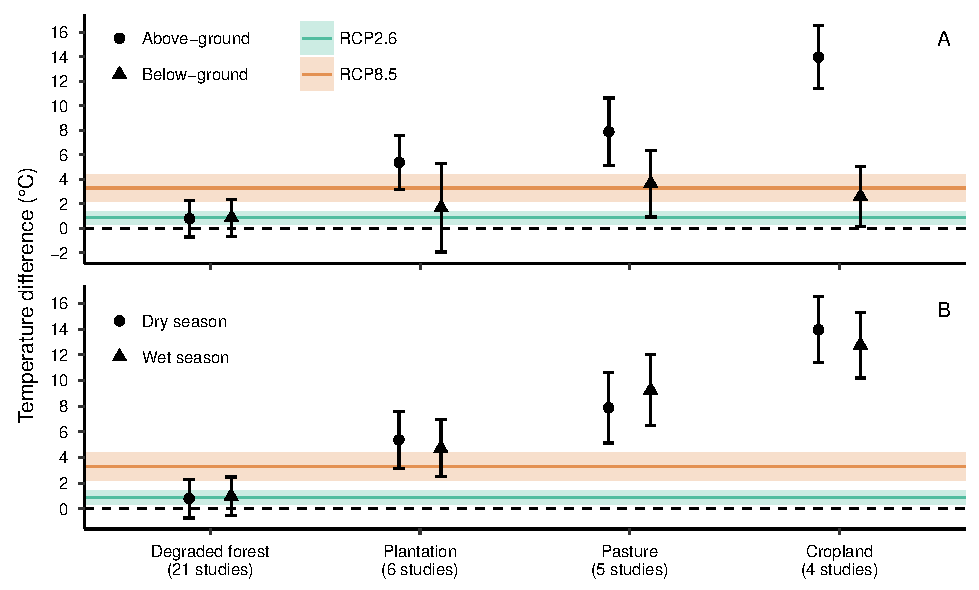
\includegraphics{figs/figA1.3.pdf}
\caption{\label{fig:fig-A-1-3}Model estimates of the temperature difference between altered land-use types and primary forest, using a reduced dataset to balance sample sizes between the different studies that contributed data. Parameter estimates are standardised against the estimate for primary forest, which is represented by the dashed line. Error bars are 95\% confidence intervals. Solid lines indicate projected warming in the tropics for the period 2081-2100 compared to the period 1986-2005, as a result of global climate change \citep{ipcc_2013}. Shaded bands indicate 5\%–95\% ranges from the distribution of the climate model ensemble. Colours represent the lowest and highest warming scenarios (RCP2.6 and RCP8.5, respectively).}
\end{figure}

\begin{figure}
\centering
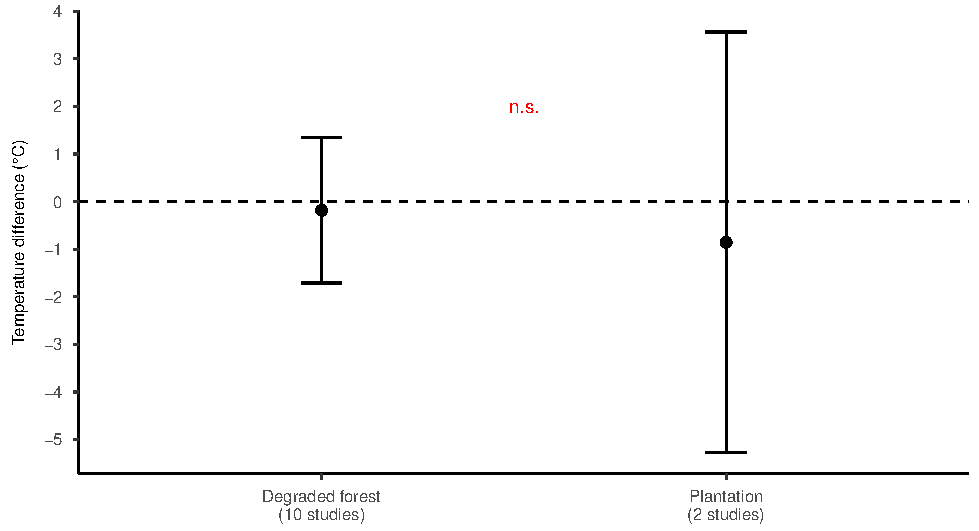
\includegraphics{./output/fig-A-1-4-1.pdf}
\caption{\label{fig:fig-A-1-4}Model estimates of the nocturnal temperature
difference between altered land-use types and primary forest. Note that
cropland and pasture are missing from this analysis because nocturnal
temperature data for these land-use types were not available. Parameter
estimates are standardised against the estimate for primary forest,
which is represented by the dotted line. Error bars are 95\% confidence
intervals.}
\end{figure}

\begin{figure}
\centering
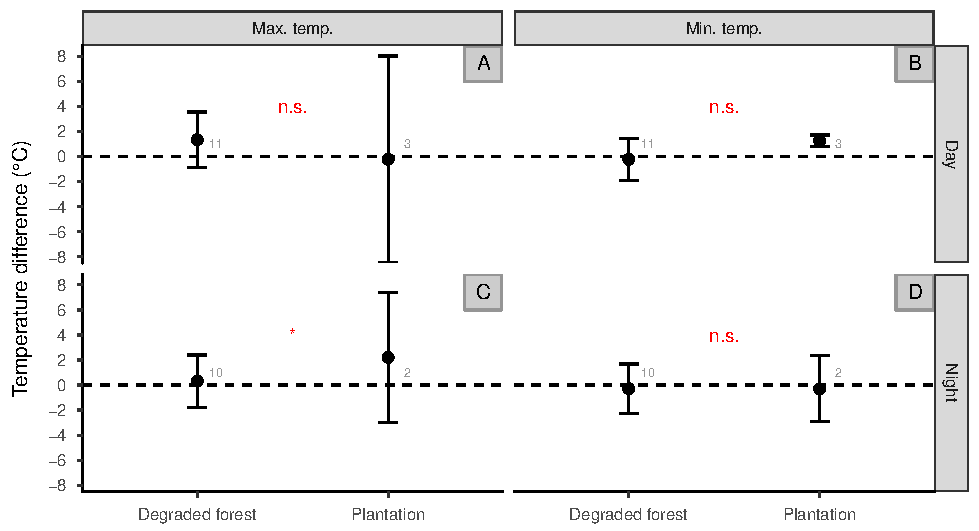
\includegraphics{./output/fig-A-1-5-1.pdf}
\caption{\label{fig:fig-A-1-5}Model estimates of the difference between
altered land-use types and primary forest in terms of temperature
extremes. Day-time results are depicted in panels A and B, and
night-time results in panels C and D. Panels A and C indicate the effect
of land-use change on maximum temperature, and panels B and D indicate
the same for minimum temperature. Note that data for cropland and
pasture are absent from this analysis because data for these land-use
types were not available. Parameter estimates are standardised against
the estimate for primary forest, which is represented by the dotted
line. Error bars are 95\% confidence intervals. The grey numbers next to
points represent the number of studies providing the underlying data.}
\end{figure}

\chapter{Supporting information for Chapter
4}\label{supporting-information-for-chapter-4}

\section{Impact of unbalanced
sampling}\label{impact-of-unbalanced-sampling}

\subsection{Methods}\label{methods-2}

Some studies contributed substantially more temperature observations
than others. To test whether these studies were unduly influencing our
results, we established a threshold over which a given land-use type, in
a given study, was deemed to have a disproportionate number of
associated temperature observations. The threshold used --- 2,071
observations --- was the mean number of observations across all unique
combinations of land-use type and study identity (55 in total). The same
number of observations (2,071) was then randomly re-sampled from each of
the land-use type and study combinations that exceeded the threshold.
With this reduced and more balanced dataset we repeated the main
analysis (see `Statistical analysis' in main text for more details),
modelling local day-time temperature (`temp\_day') against land-use type
(`LUT'), position relative to ground-level (`position') and season. The
final model structure was unchanged, and included a random slope for
land-use type and random intercept with respect to the identity of the
study (`studyID') from which data originated:

\texttt{lmer(temp\_day\ \ \textasciitilde{}\ LUT*position\ +\ LUT*season\ +\ (LUT\textbar{}studyID))}

\subsection{Results}\label{results-3}

All results were qualitatively unchanged from those derived using the
full dataset. Local day-time temperature was warmer in altered land-use
types, compared to primary forest (LMM, Χ\textsuperscript{2} = 32.19, df
= 4, P \textless{} 0.001; \autoref{fig:fig-A-1-3}). Averaged across
above- and below-ground, and across seasons, the temperature
differential was greatest in cropland (7.7°C), followed by pasture
(6.4°C), plantation (3.2°C) and degraded forest (0.9°C). The
relationship between land-use type and temperature interacted with both
position relative to ground level (LMM, Χ\textsuperscript{2} = 681, df =
4, P \textless{} 0.001; \autoref{fig:fig-A-1-3}A) and season (LMM,
Χ\textsuperscript{2} = 105.63, df = 4, P \textless{} 0.001;
\autoref{fig:fig-A-1-3}B). Specifically, the difference between altered
land-use types and primary forest was greater above-ground than
below-ground (\autoref{fig:fig-A-1-3}A), and variable between seasons
according to the land-use type (\autoref{fig:fig-A-1-3}B).

\pagebreak

\section{Supplementary figures}\label{supplementary-figures-1}

\begin{figure}
\centering
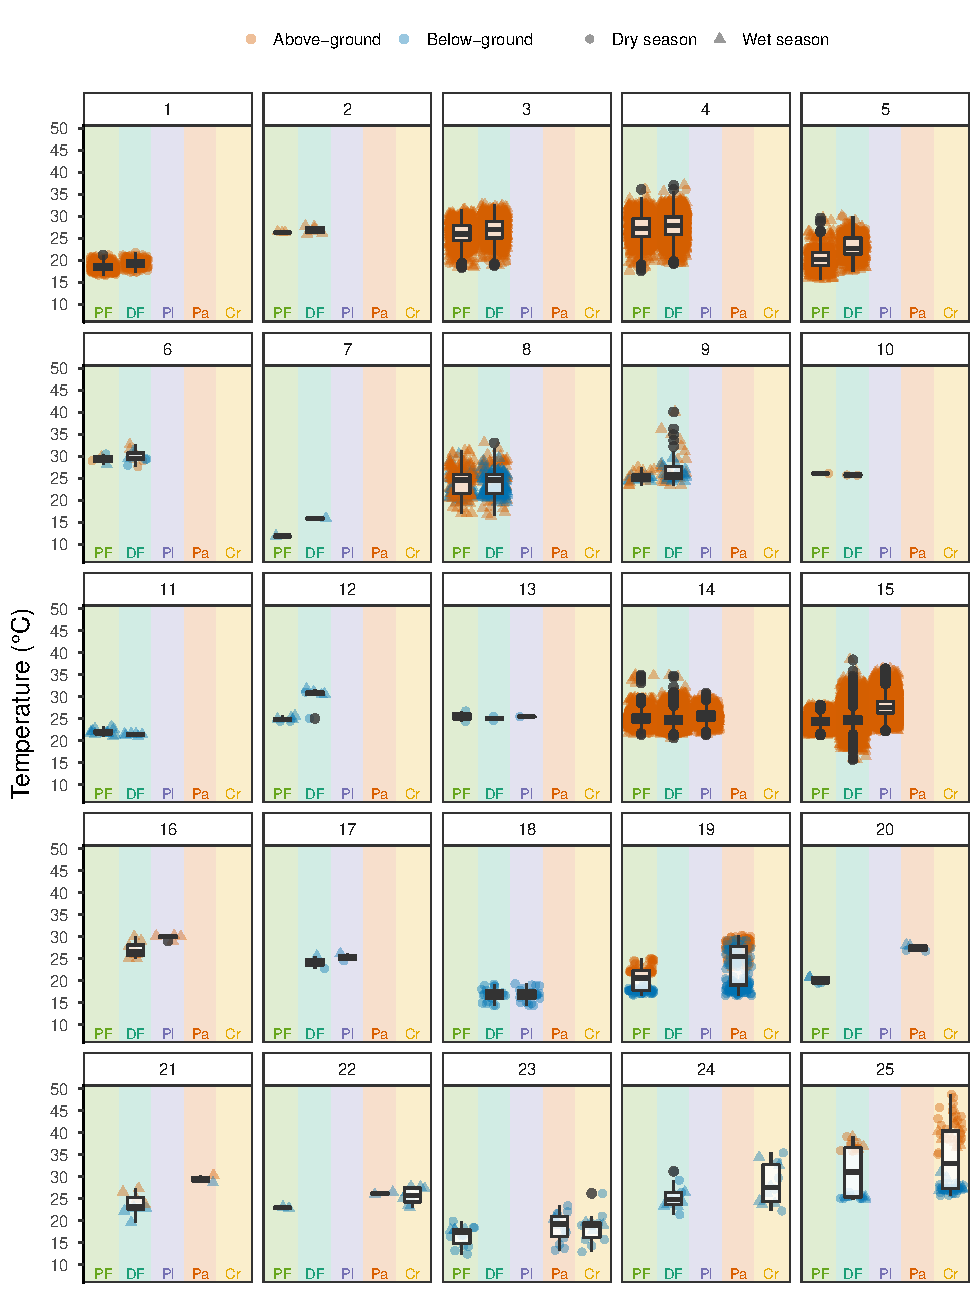
\includegraphics{./output/fig-A-1-1-1.pdf}
\caption{\label{fig:fig-A-1-1}Day-time temperature against land-use type for
each study contributing data to the analyses. Panel numbers refer to the
study number in the reference list below. Land-use types are: primary
forest (PF), degraded forest (DF), plantation (Pl), pasture (Pa) and
cropland (Cr). Panels are ordered by the combination of land-use types
for which data was available: (1-12) PF + DF; (13-15) PF + DF + Pl;
(16-18) DF + Pl; (19-20) PF + Pa; (21) DF + Pa; (22-23) PF + Pa + Cr;
and (24-25) DF + Cr. Shading of points indicates temperatures measured
above-ground (orange) or below-ground (blue), and point symbol indicates
temperatures measured during the dry season (circles) or wet season
(triangles).}
\end{figure}

\begin{figure}
\centering
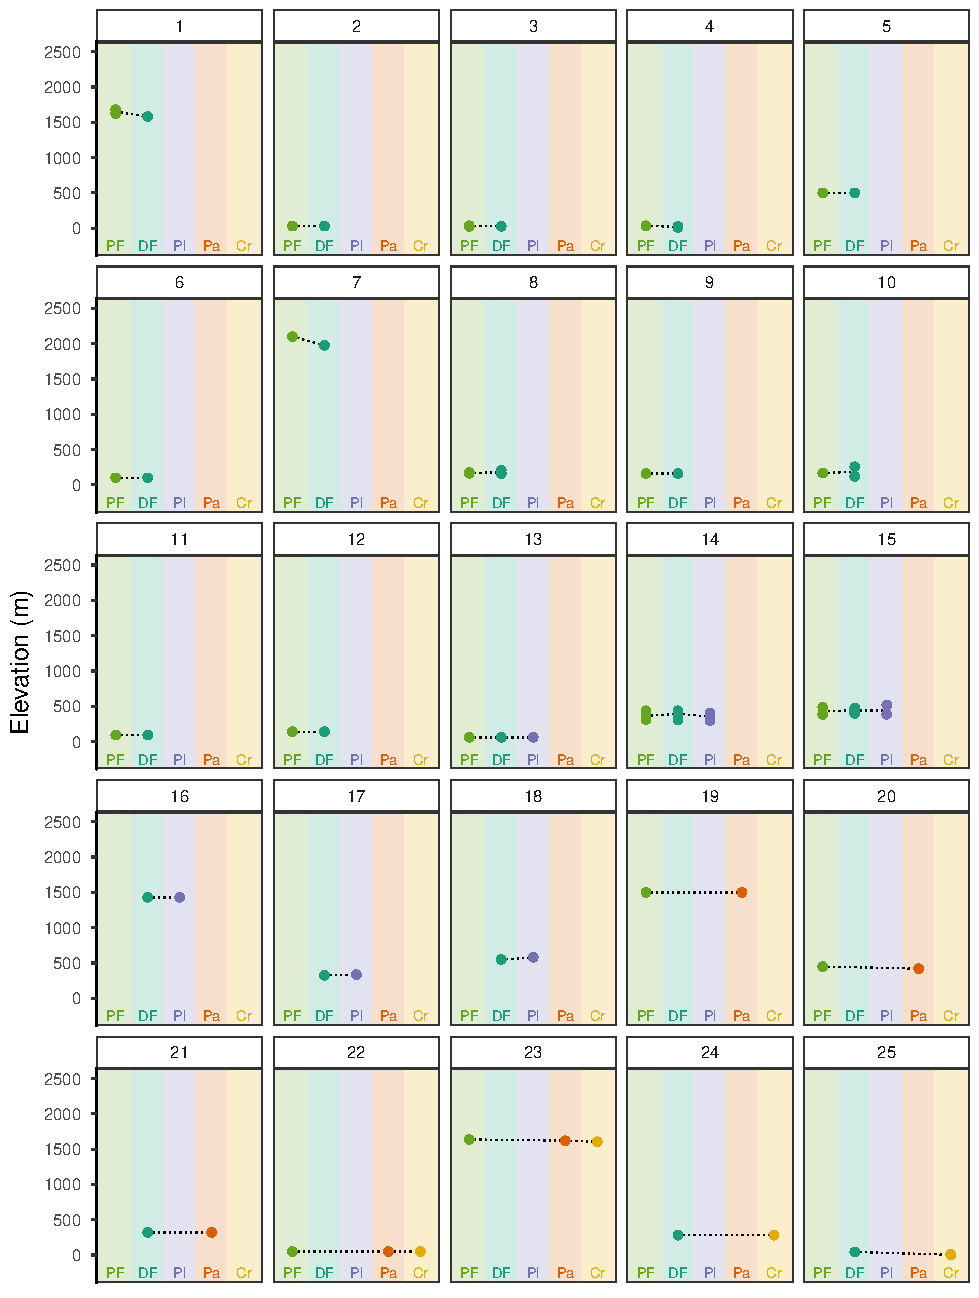
\includegraphics{./output/fig-A-1-2-1.pdf}
\caption{\label{fig:fig-A-1-2}Site elevation against land-use type for each
study contributing data to the analyses. Panel numbers refer to the
study number in the reference list below. Land-use types are: primary
forest (PF), degraded forest (DF), plantation (Pl), pasture (Pa) and
cropland (Cr). Panels are ordered by the combination of land-use types
for which data was available: (1-12) PF + DF; (13-15) PF + DF + Pl;
(16-18) DF + Pl; (19-20) PF + Pa; (21) DF + Pa; (22-23) PF + Pa + Cr;
and (24-25) DF + Cr. Dotted black lines connect the mean elevation of
all the sites within each land-use type.}
\end{figure}

\begin{figure}
\centering
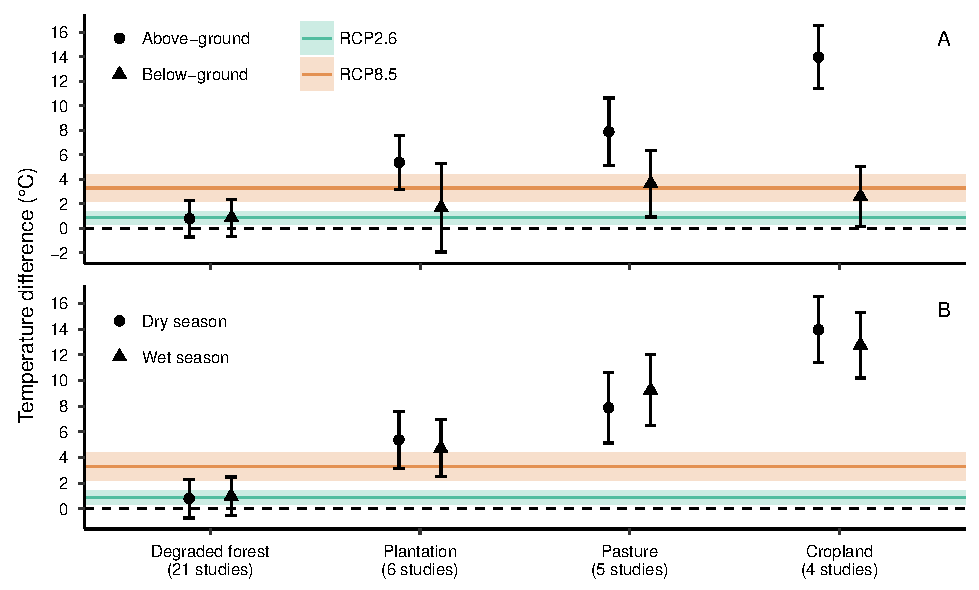
\includegraphics{figs/figA1.3.pdf}
\caption{\label{fig:fig-A-1-3}Model estimates of the temperature difference between altered land-use types and primary forest, using a reduced dataset to balance sample sizes between the different studies that contributed data. Parameter estimates are standardised against the estimate for primary forest, which is represented by the dashed line. Error bars are 95\% confidence intervals. Solid lines indicate projected warming in the tropics for the period 2081-2100 compared to the period 1986-2005, as a result of global climate change \citep{ipcc_2013}. Shaded bands indicate 5\%–95\% ranges from the distribution of the climate model ensemble. Colours represent the lowest and highest warming scenarios (RCP2.6 and RCP8.5, respectively).}
\end{figure}

\begin{figure}
\centering
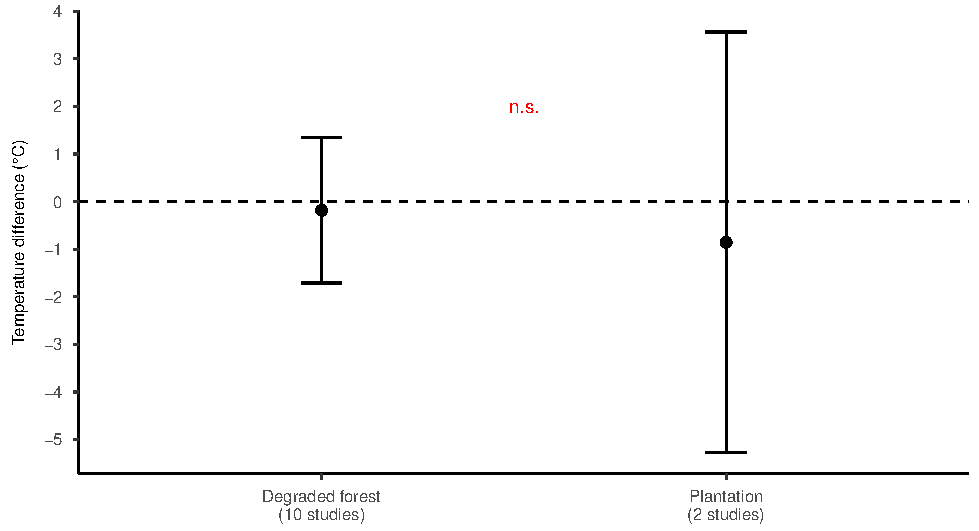
\includegraphics{./output/fig-A-1-4-1.pdf}
\caption{\label{fig:fig-A-1-4}Model estimates of the nocturnal temperature
difference between altered land-use types and primary forest. Note that
cropland and pasture are missing from this analysis because nocturnal
temperature data for these land-use types were not available. Parameter
estimates are standardised against the estimate for primary forest,
which is represented by the dotted line. Error bars are 95\% confidence
intervals.}
\end{figure}

\begin{figure}
\centering
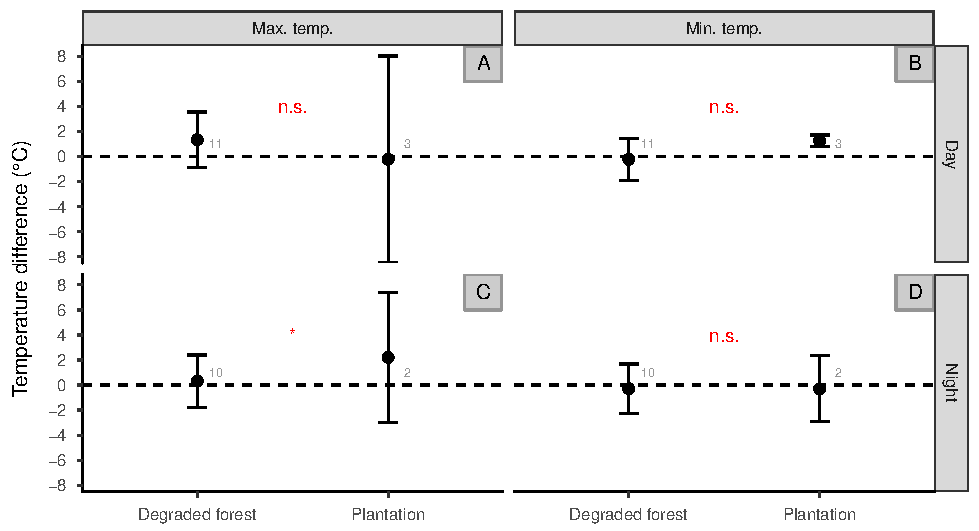
\includegraphics{./output/fig-A-1-5-1.pdf}
\caption{\label{fig:fig-A-1-5}Model estimates of the difference between
altered land-use types and primary forest in terms of temperature
extremes. Day-time results are depicted in panels A and B, and
night-time results in panels C and D. Panels A and C indicate the effect
of land-use change on maximum temperature, and panels B and D indicate
the same for minimum temperature. Note that data for cropland and
pasture are absent from this analysis because data for these land-use
types were not available. Parameter estimates are standardised against
the estimate for primary forest, which is represented by the dotted
line. Error bars are 95\% confidence intervals. The grey numbers next to
points represent the number of studies providing the underlying data.}
\end{figure}

\clearpage
\fancyhead[R]{Bibliography}

\bibliography{refs}


\end{document}
